 
To determine the efficiency of the dilepton triggers, 
we derive the efficiency of the requirements imposed on each leg separately.
This requires a modification to the tag and probe method described above in some cases.
If the trigger objects are saved by the HLT before the requirement that there be two valid objects then
we can check each leg independently of the other using the usual tag and probe method.
If the trigger objects are saved after the requirement that there are two valid objects, then there is 
a 100\% correlation between the decision we can probe on each lepton.
This means that we must pick exactly one tag candidate for each event a priori, which we do 
randomly. 
If the randomly selected tag candidate meets the tight requirements then we are free to 
probe the other lepton.

%\subsubsection{Electron triggers}
%%%%%% double
The double electron trigger requires the higher $p_T$ leg to be seeded at Level-1.
The efficiency of the seeded leg with respect to a denominator object above the 
triggr $p_T$ threshold was found to be $0.993^{+0.001}_{-0.001}$ in the barrel and
$0.994^{+0.002}_{-0.003}$ in the endcap.
%The per electron efficiency with respect to electrons passing the offline selection
%is shown for the seeded leg in  
%Figure \ref{fig:Ele17Ele8TriggerEfficiencySeededLeg} as a function of $p_{T}$ and $\eta$, 
%and the unseeded leg in Figure \ref{fig:Ele17Ele8TriggerEfficiencyUnseededLeg}.
%The results are summarised in Table \ref{tab:eff_double_ele}. 
The per electron efficiency for the unseeded leg of 
HLT\_Ele17\_CaloIdL\_CaloIsoVL\_Ele8\_CaloIdL\_CaloIsoVL\_v*
is given in Table \ref{tab:eff_ele_17_8_A} and for\\
HLT\_Ele17\_\{CaloIdT\_TrkIdVL\_CaloIsoVL\_TrkIsoVL\}\_Ele8\_\{X\}\_v* in
Table \ref{tab:eff_ele_17_8_B}.
The double muon trigger {HLT\_DoubleMu7 } requires both legs to be seeded at Level-1.
The per muon efficiency for each leg of the double muon trigger is
summarized in Table \ref{tab:eff_mu_7_7}.

\begin{table}[!ht]
\begin{center}
\begin{tabular}{c|c|c}
\hline
Measurement & Barrel ( $|\eta|<1.5$ )   & Endcap ( $|\eta|>1.5$ )  \\ 
\hline
$  10<p_T<  15$ & 0.97 $\pm$ 0.01  & 1.00 $\pm$ 0.02  \\ \hline 
$  15<p_T<  20$ & 0.99 $\pm$ 0.00  & 1.00 $\pm$ 0.00  \\ \hline 
$  20<p_T<  50$ & 1.00 $\pm$ 0.00  & 1.00 $\pm$ 0.00  \\ \hline 
\end{tabular}
\caption{The efficiency for HLT\_Ele17\_CaloIdL\_CaloIsoVL\_Ele8\_CaloIdL\_CaloIsoVL\_v* (runs 160329-).}
\label{tab:eff_ele_17_8_A}
\end{center}
\end{table}

\begin{table}[!ht]
\begin{center}
\begin{tabular}{c|c|c}
\hline
Measurement & Barrel ( $|\eta|<1.5$ )   & Endcap ( $|\eta|>1.5$ )  \\ 
\hline
$  10<p_T<  15$ & 0.97 $\pm$ 0.01  & 1.00 $\pm$ 0.02  \\ \hline 
$  15<p_T<  20$ & 0.99 $\pm$ 0.00  & 1.00 $\pm$ 0.00  \\ \hline 
$  20<p_T<  50$ & 1.00 $\pm$ 0.00  & 1.00 $\pm$ 0.00  \\ \hline 
\end{tabular}
\caption{The efficiency for HLT\_Ele17\_CaloIdL\_CaloIsoVL\_Ele8\_CaloIdL\_CaloIsoVL\_v* (runs 160329-).}
\label{tab:eff_ele_17_8_B}
\end{center}
\end{table}

%\begin{figure}[!ht]
%\begin{center}
%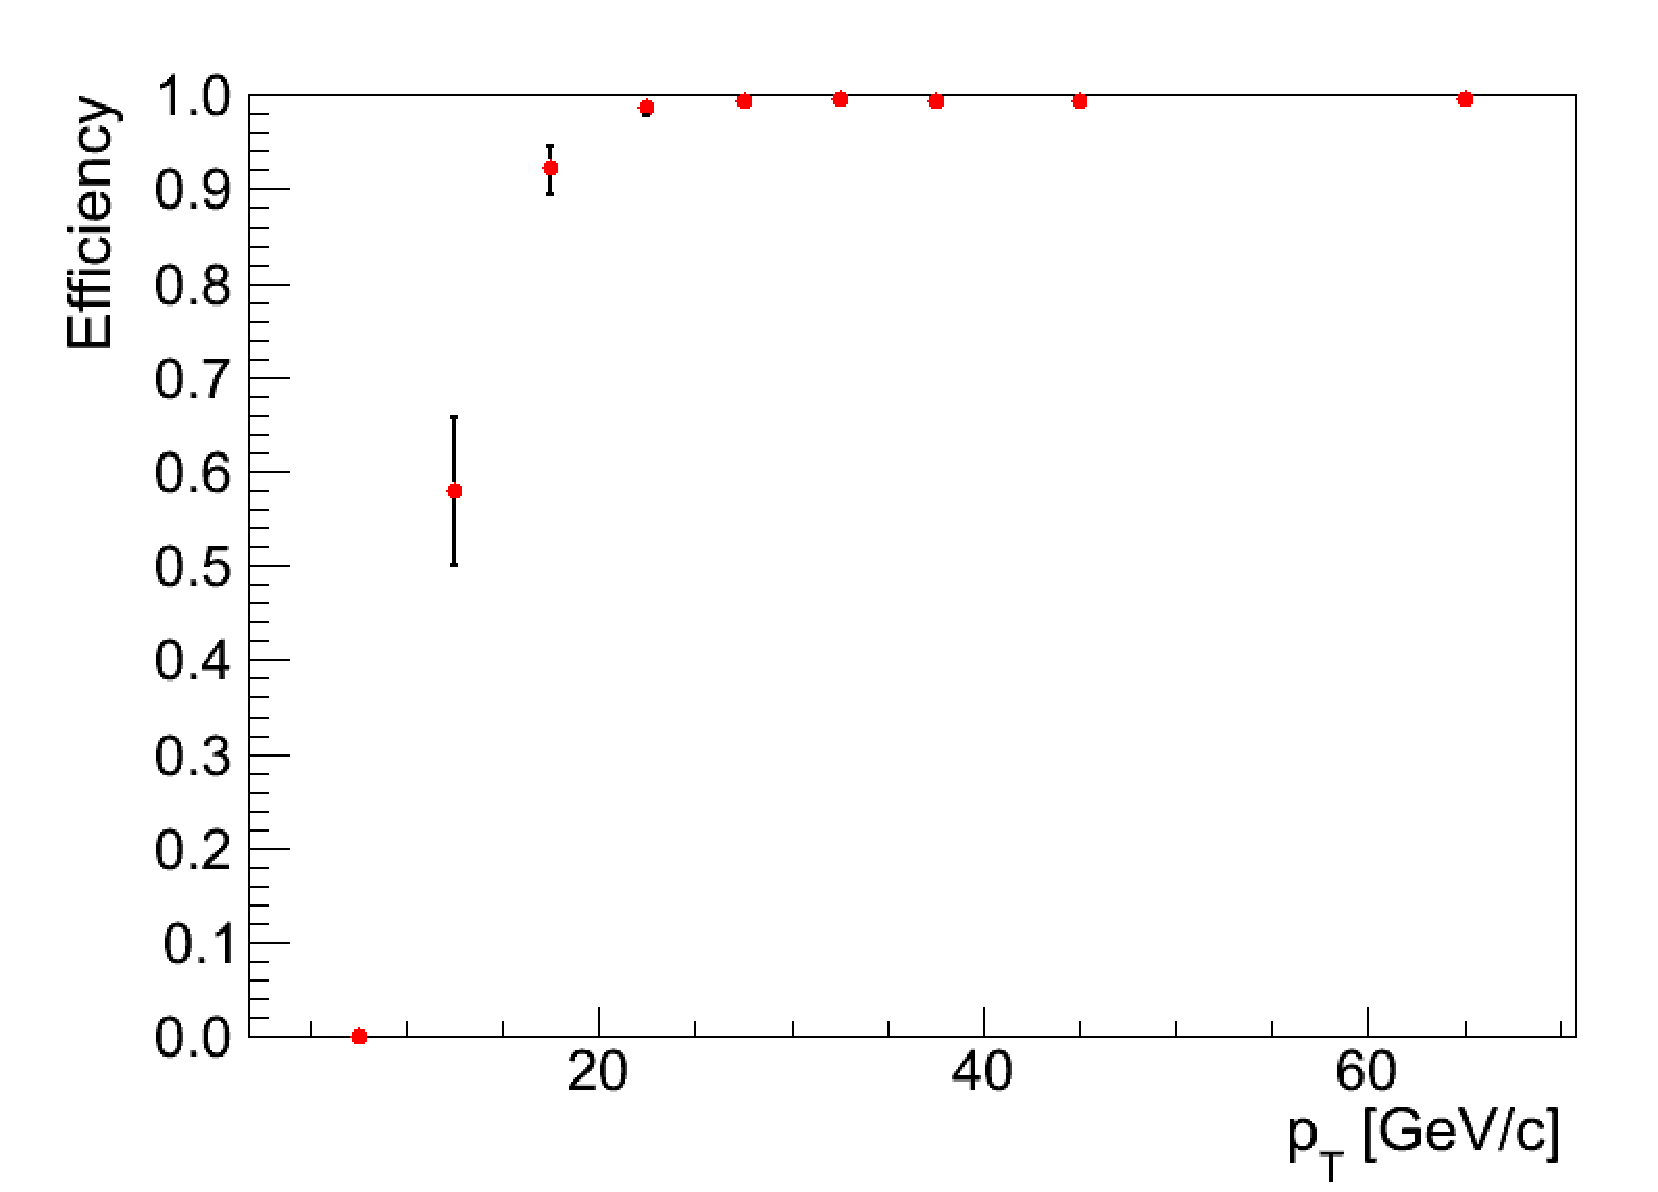
\includegraphics[width=0.48\textwidth]{figures/ElectronTriggerEffVsPt_Ele17Ele8WithL1Seed.pdf}
%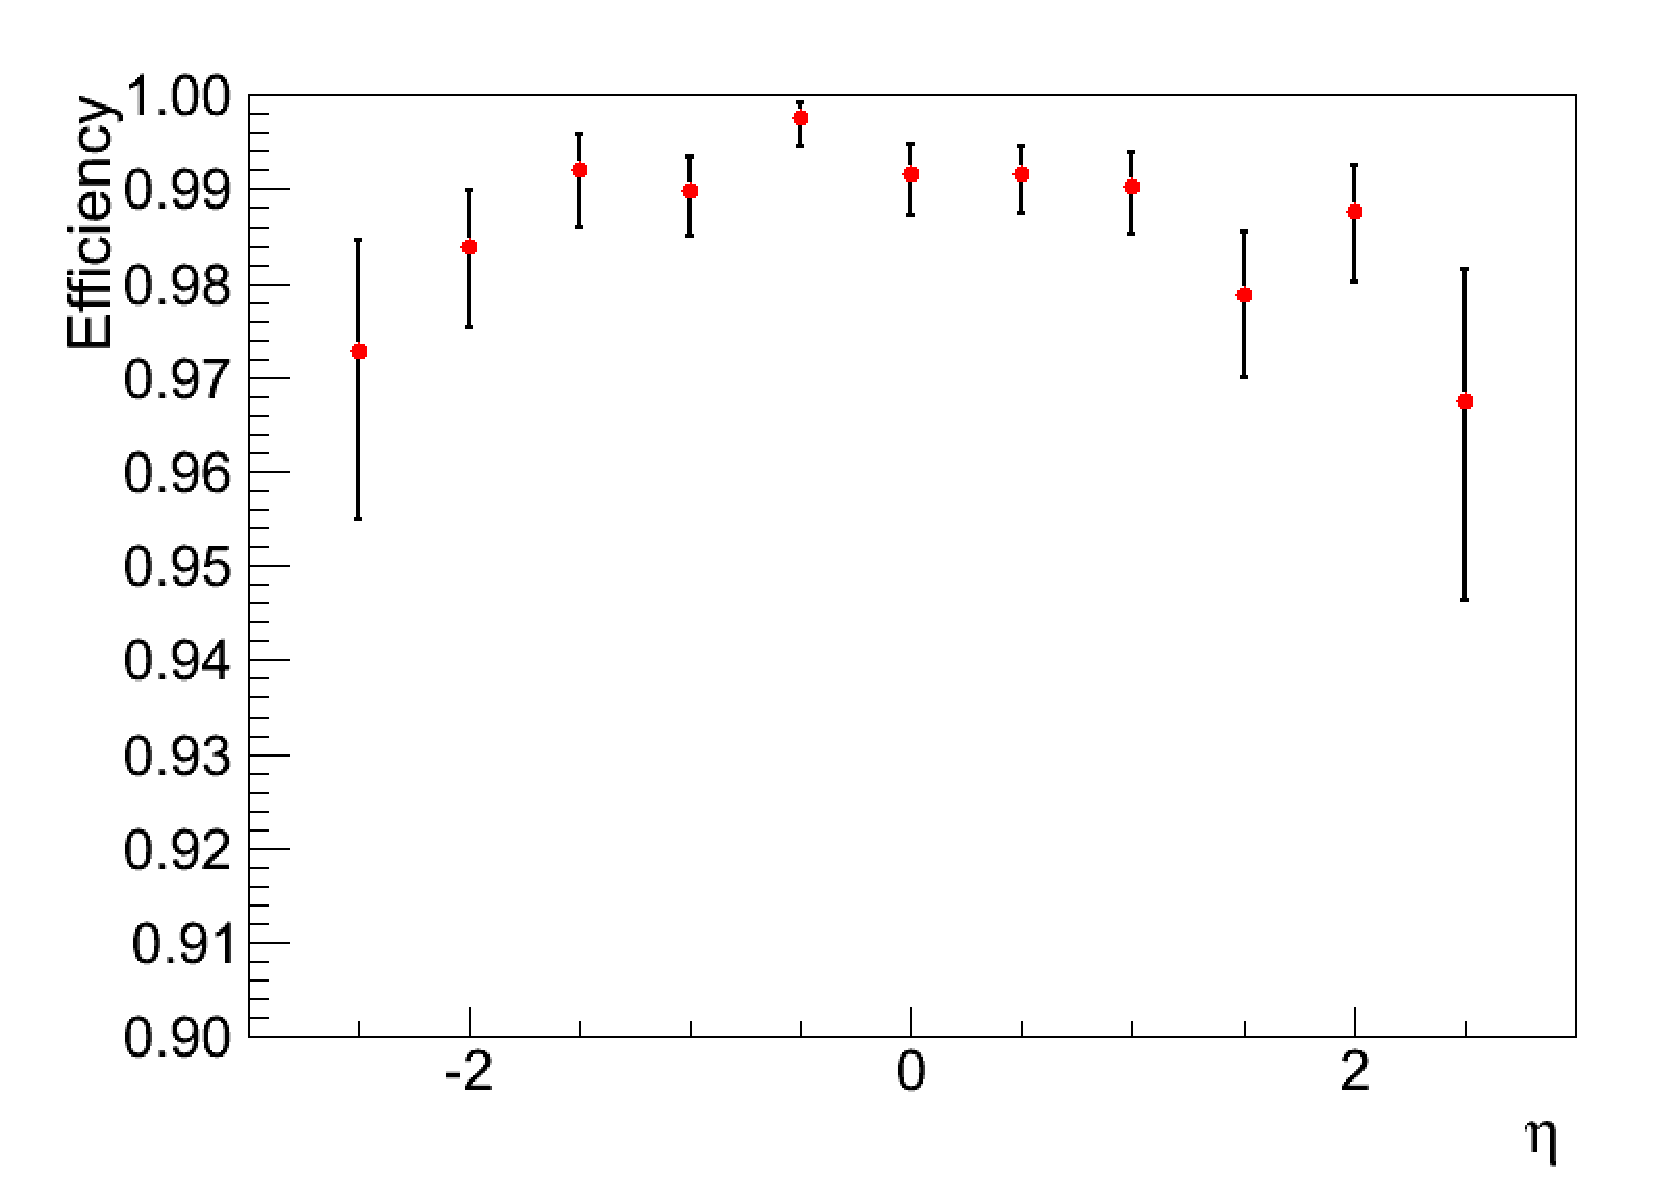
\includegraphics[width=0.48\textwidth]{figures/ElectronTriggerEffVsEta_Ele17Ele8WithL1Seed.pdf}
%\end{center}
%\caption{Efficiency for the L1 seeded leg of the double electron trigger as a function of $p_{T}$ (a) and $\eta$ (b).}
%\label{fig:Ele17Ele8TriggerEfficiencySeededLeg}
%\end{figure} 
%\begin{figure}[!ht]
%\begin{center}
%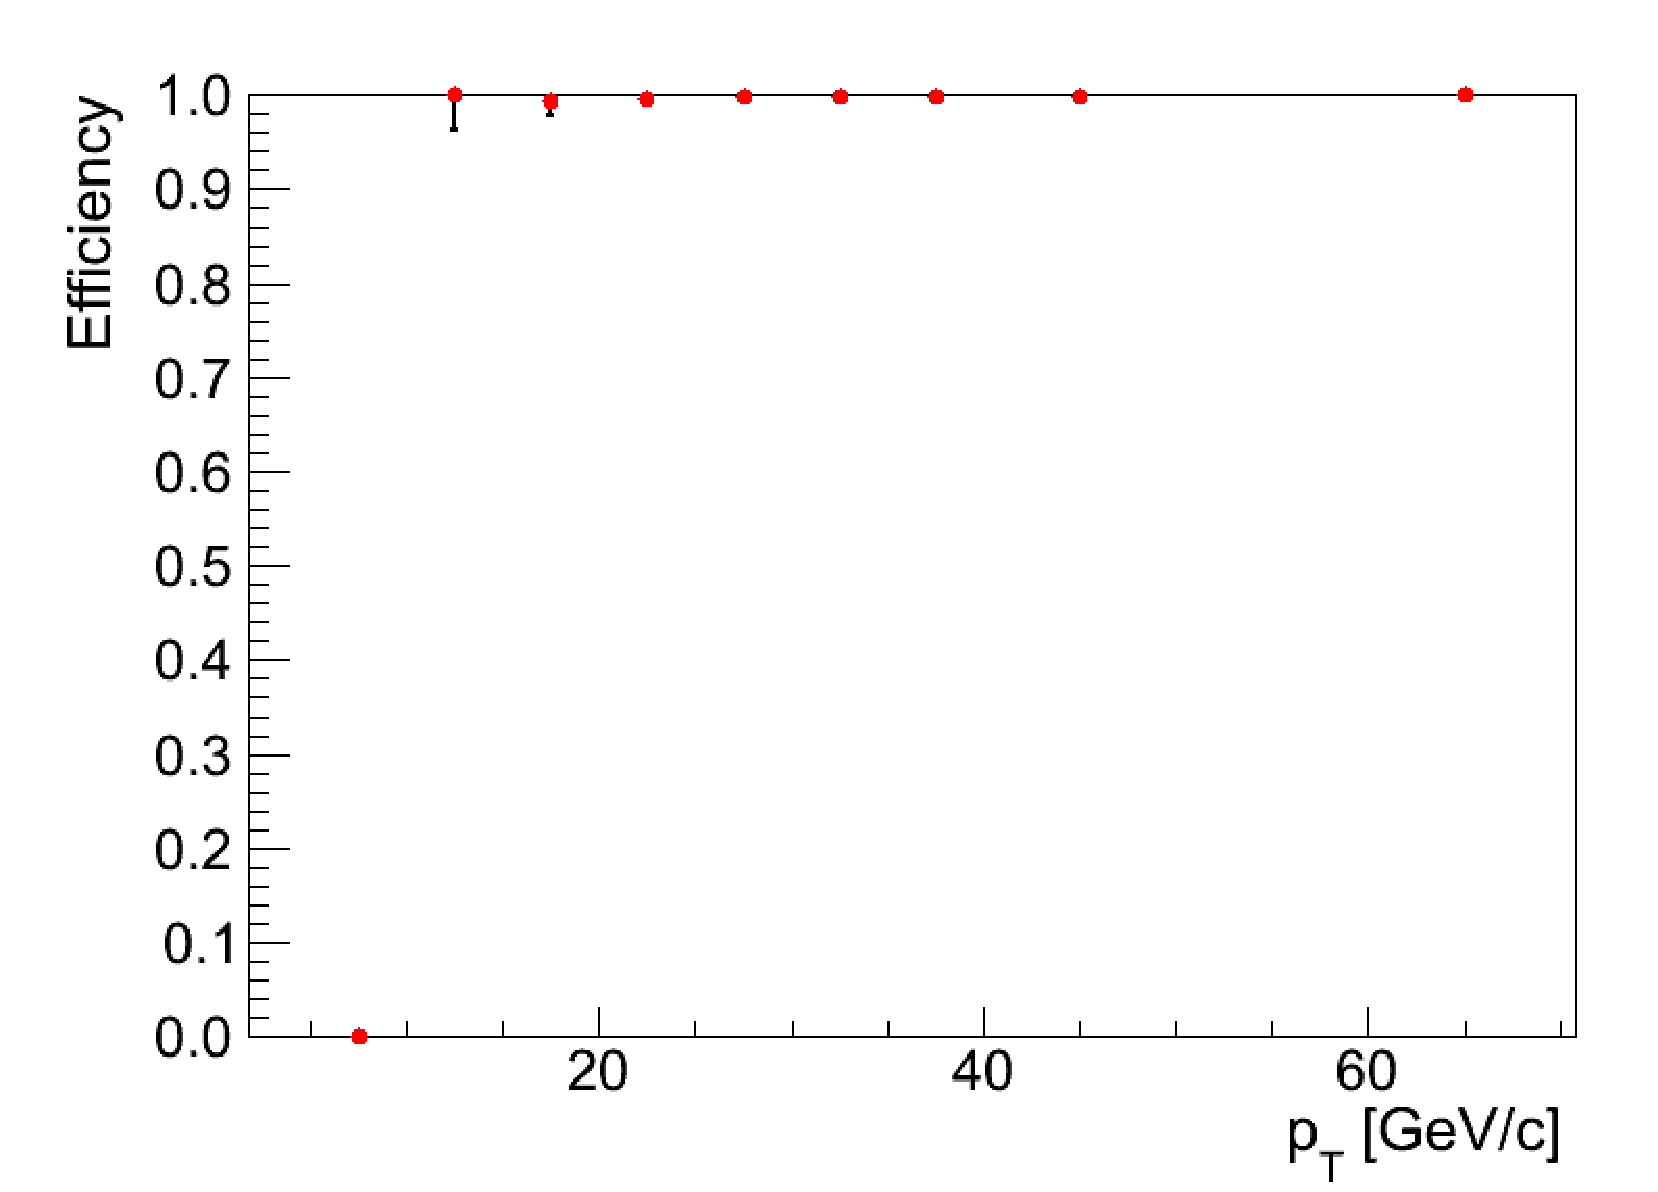
\includegraphics[width=0.48\textwidth]{figures/ElectronTriggerEffVsPt_Ele17Ele8.pdf}
%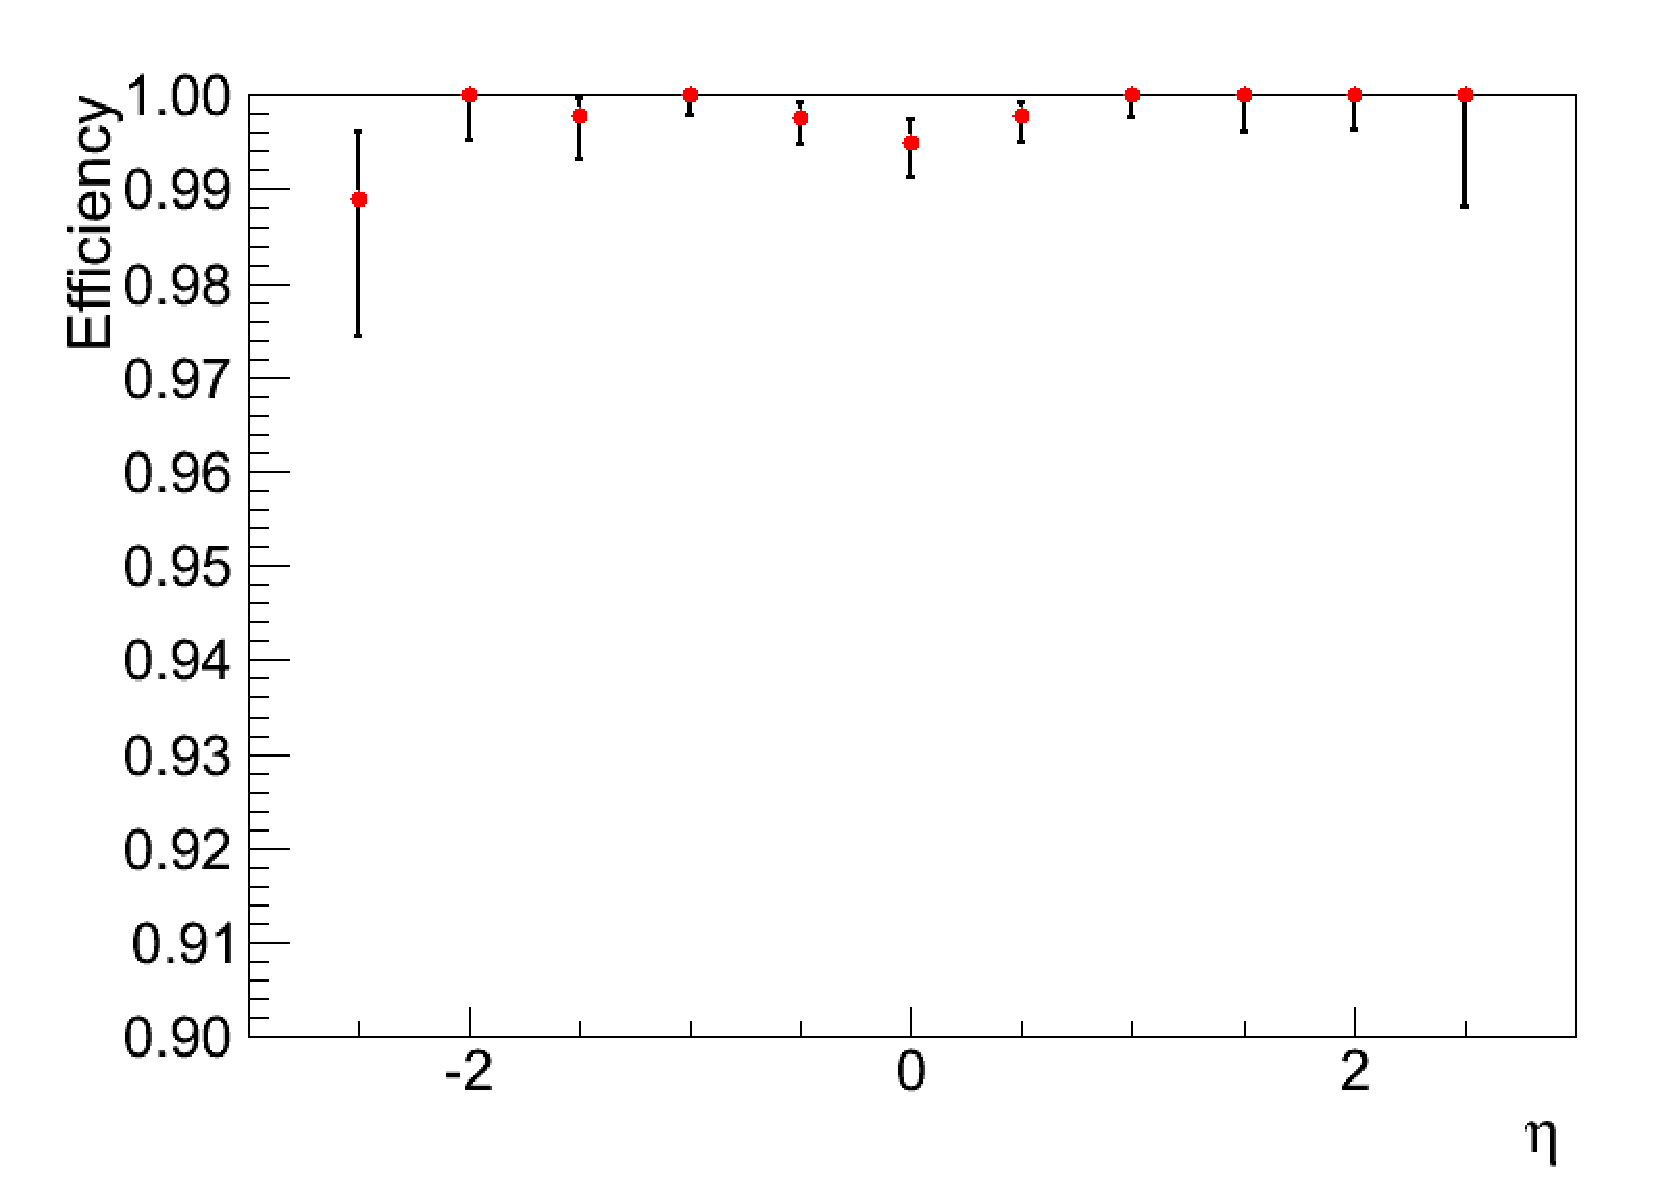
\includegraphics[width=0.48\textwidth]{figures/ElectronTriggerEffVsEta_Ele17Ele8.pdf}
%\end{center}
%\caption{Efficiency for the unseeded leg of the double electron trigger as a function of $p_{T}$ (a) and $\eta$ (b).}
%\label{fig:Ele17Ele8TriggerEfficiencyUnseededLeg}
%\end{figure}
%
%\begin{table}[!ht]
%\begin{center}
%\begin{tabular}{c|c|c} \hline
%              & Barrel ( $|\eta|<1.5$ )  & Endcap ( $|\eta|>1.5$ )  \\  \hline
%\hline
%Seeded Leg 20$<p_{T}$   & 0.9931 + 0.0012 - 0.0014 & 0.9942 + 0.0019 - 0.0026 \\ \hline
%Unseeded Leg 10$<p_{T}<$15 & 1.0 + 0.0 - 0.07 & 1.0 + 0.0 - 0.08                 \\ \hline
%Unseeded Leg 15$<p_{T}<$20 & 1.0 + 0.0 - 0.02 & 0.985 + 0.012 - 0.033            \\ \hline
%Unseeded Leg 20$<p_{T}$   & 0.9981 + 0.0006 - 0.0009 & 0.9993 + 0.0005 - 0.0015 \\
%\hline
%\end{tabular}
%\caption{Efficiency for the seeded and unseeded legs of the double electron trigger 
%separately in bins of $p_{T}$ for the barrel and endcap.
%\label{tab:eff_double_ele}}
%\end{center}
%\end{table}
%%%%%% single
%
%The per electron efficiency for the
%single electron trigger with respect to electrons passing the offline selection
%is shown in Figure \ref{fig:Ele27Efficiency} and summarized
%in Table \ref{tab:Ele27Efficiency}.
%
%\begin{figure}[!ht]
%\begin{center}
%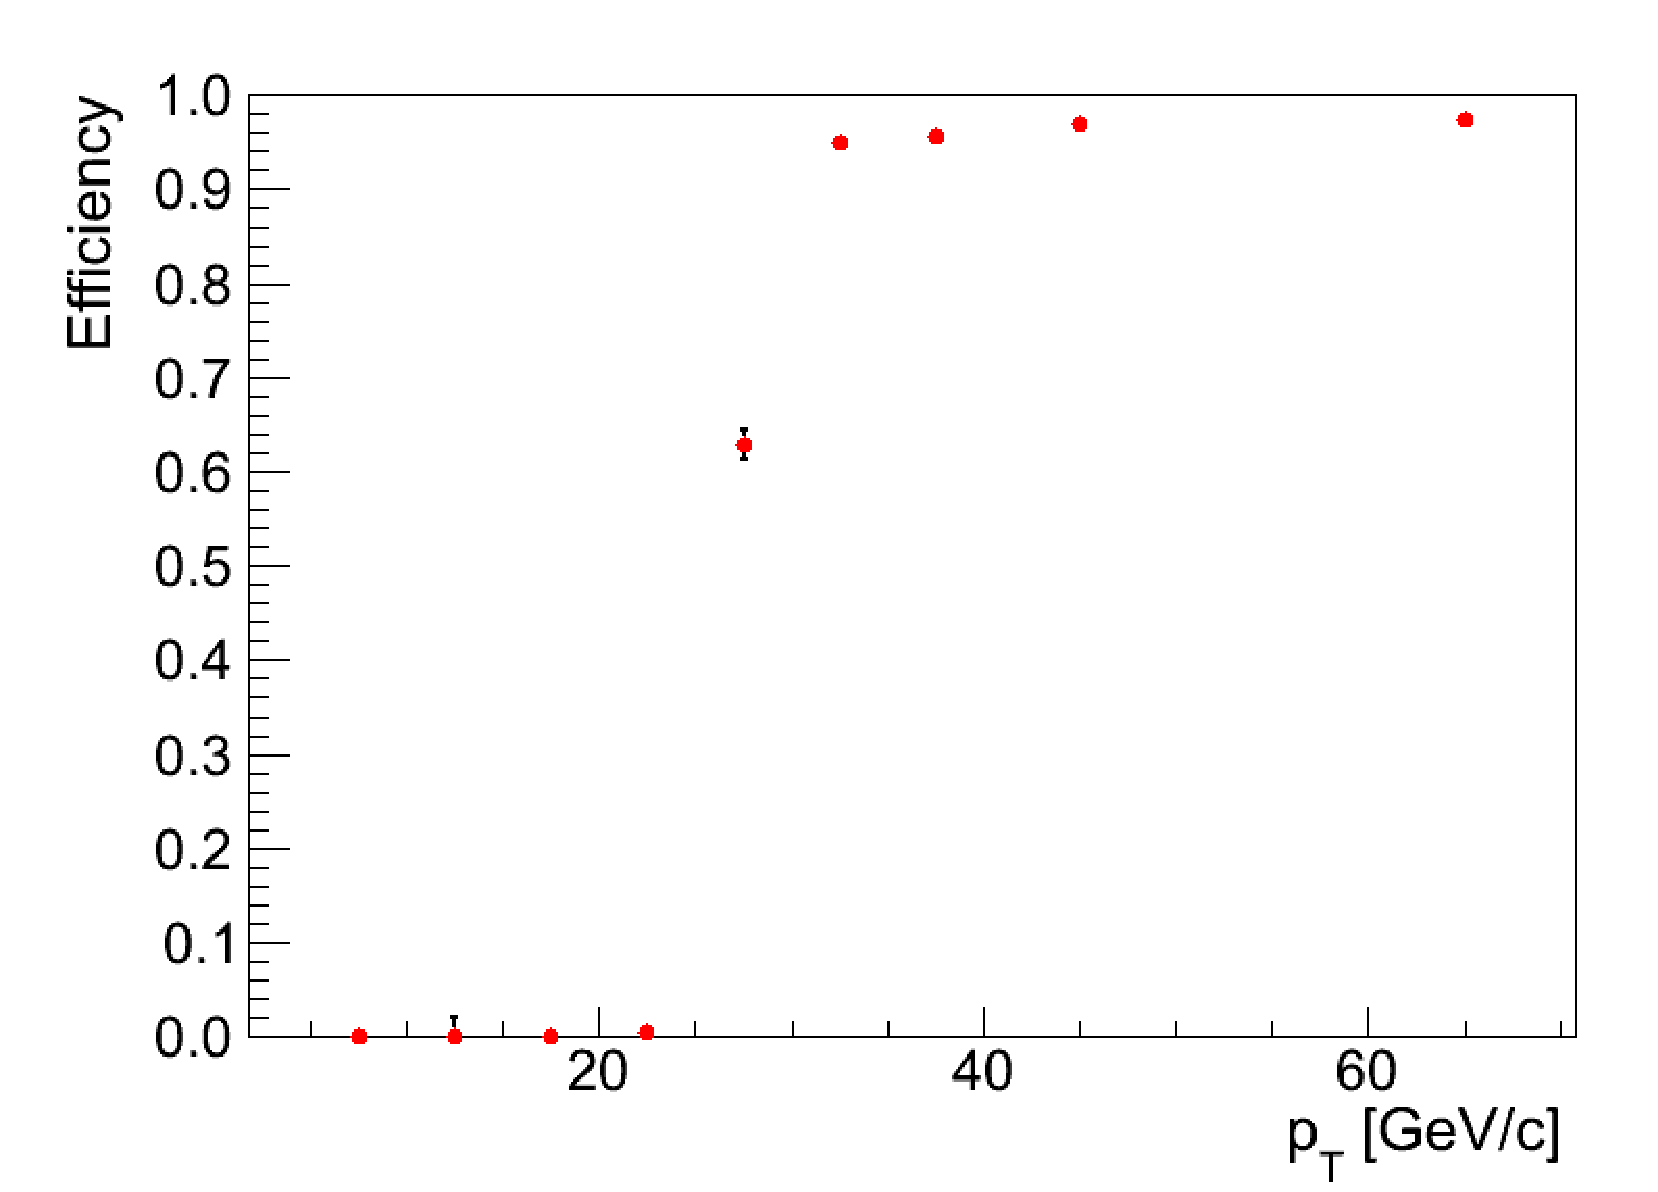
\includegraphics[width=0.48\textwidth]{figures/ElectronTriggerEffVsPt_Ele27Tight.pdf}
%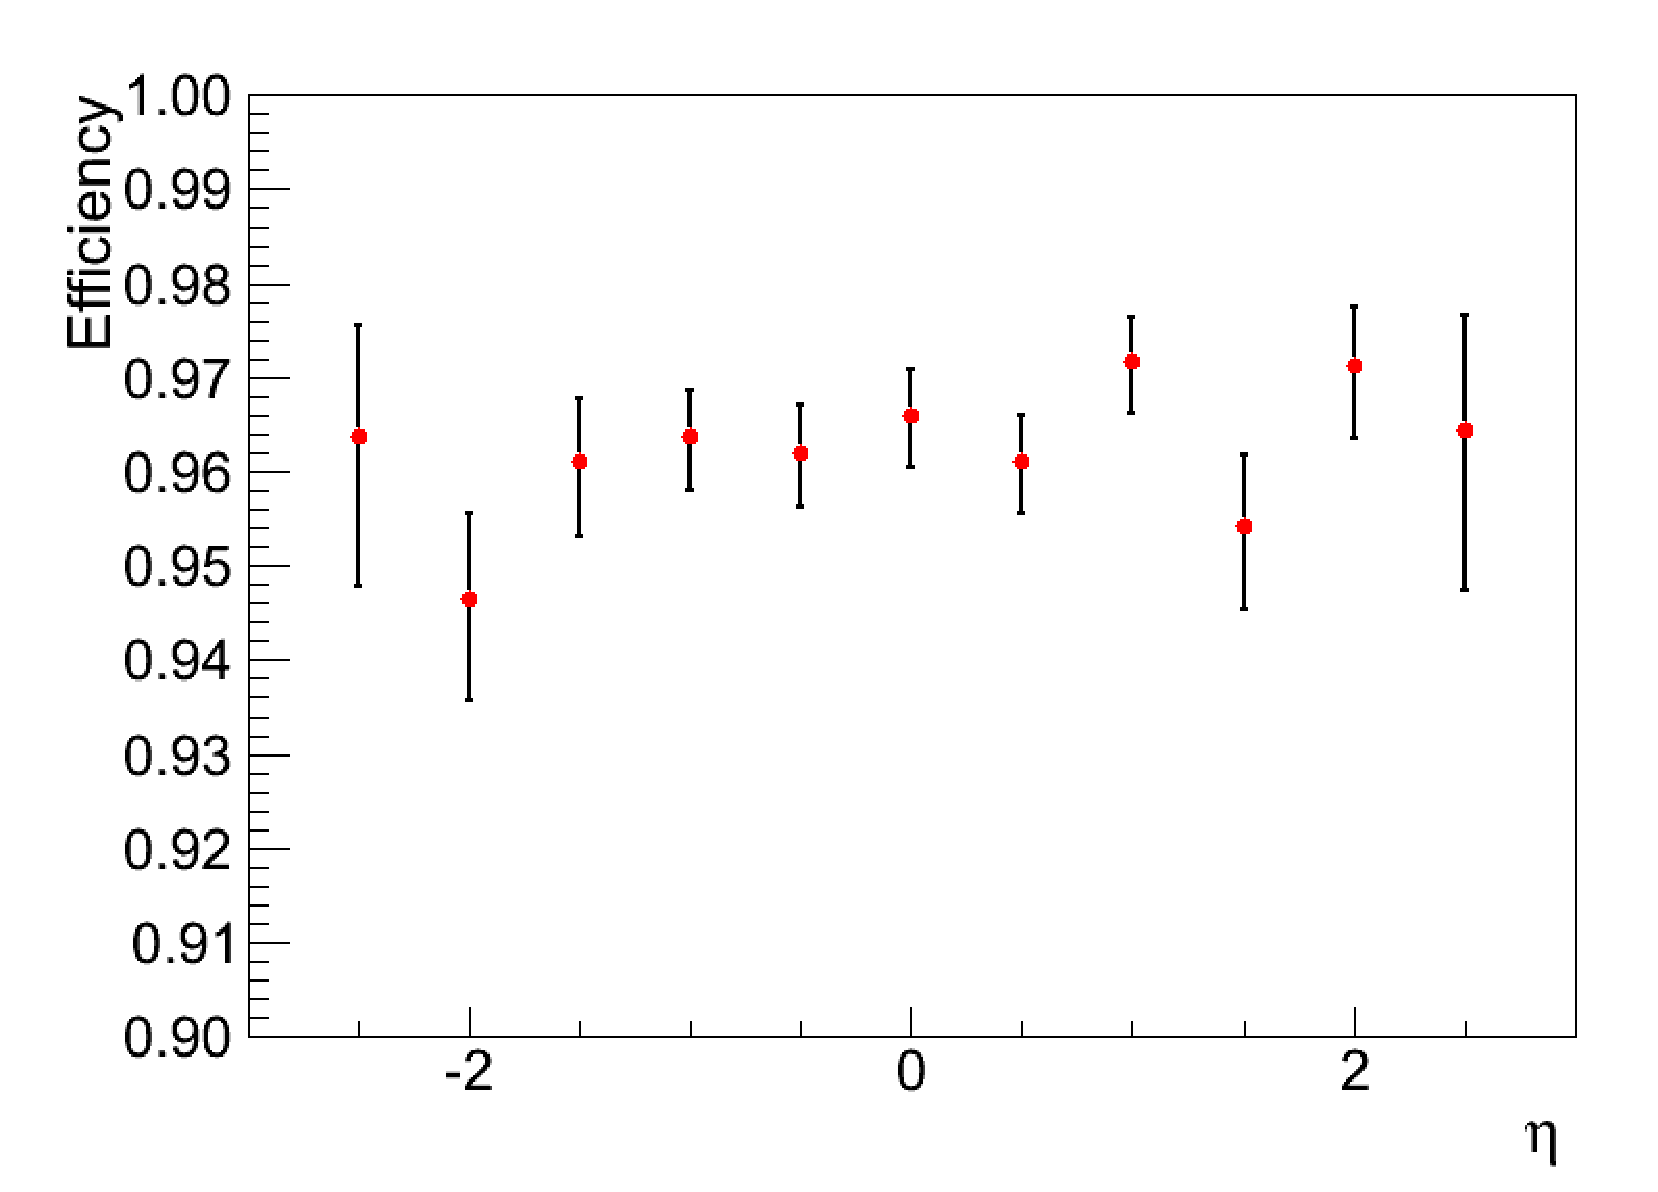
\includegraphics[width=0.48\textwidth]{figures/ElectronTriggerEffVsEta_Ele27Tight.pdf}
%\end{center}
%\caption{The single leg efficiency of the single electron trigger as a function of $p_{T}$ (a) and $\eta$ (b).}
%\label{fig:Ele27Efficiency}
%\end{figure}

%\begin{table}[!ht]
%\begin{center}
%\begin{tabular}{c|c|c} \hline
%              & Barrel ( $|\eta|<1.5$ )  & Endcap ( $|\eta|>1.5$ )  \\  \hline
%\hline
%30$<p_{T}$   & 0.964 + 0.002 - 0.002 & 0.958 + 0.004 - 0.004 \\
%\hline
%\end{tabular}
%\caption{The single leg efficiency of the single electron trigger 
%separately in bins of $p_{T}$ for the barrel and endcap.
%\label{tab:Ele27Efficiency}}
%\end{center}
%\end{table}
%
%
%
%
%\subsubsection{Muon triggers}
%
%The trigger efficiencies are plotted as a function of the $p_{T}$ and $\eta$ of the
%muon candidate in Fig \ref{fig:SingleMu15TriggerEfficiency} and 
%\ref{fig:SingleIsoMu17TriggerEfficiency} for the single muon and 
%isolated single muon triggers respectively. 
%
% REMARK: DLE - this is a good point and I forgot about it.  Should repeat.
% But for now... Sigh... How in the world to take it into account correctly
% when re-weighting MC...
%
%We show the single muon trigger efficiencies for two periods of data taking,
%because the first period was affected by a bug in the Level-1 trigger logic,
%which is clearly visible as an inefficiency in the negative endcap region.

\begin{table}[!ht]
\begin{center}
\begin{tabular}{c|c|c}
\hline
Measurement & Barrel ( $|\eta|<1.5$ )   & Endcap ( $|\eta|>1.5$ )  \\ 
\hline
$  10<p_T<  15$ & 0.95 $\pm$ 0.02  & 0.94 $\pm$ 0.02  \\ \hline 
$  15<p_T<  20$ & 0.98 $\pm$ 0.01  & 0.97 $\pm$ 0.01  \\ \hline 
$  20<p_T<  50$ & 0.96 $\pm$ 0.00  & 0.96 $\pm$ 0.00  \\ \hline 
\end{tabular}
\caption{The efficiency for HLT\_DoubleMu7.}
\label{tab:eff_mu_7_7}
\end{center}
\end{table}

In the case of the $e\mu$ triggers, the efficiency of the muon leg can be
taken from the appropriate bin of Table \ref{tab:eff_mu_7_7} because the 
requirements other than the $p_T$ threshold are the same.
In the case of the electron leg, the requirements applied are looser
to those of the double electron triggers.
The efficiency of the electron leg was cross checked using $t\bar{t}$ 
events in the $e\mu$ final state using the tag
and probe method described previously.
In this case the tag was required to be a muon passing the muon part of the
trigger, and the probe was an electron passing the offline selection.
To select a well defined $t\bar{t}$ event sample, the MET was required to be
above $20~GeV$.
The results were consistant with the other double electron triggers.

%, and plotted in 
%Fig. \ref{fig:DoubleMu7TriggerEfficiency} as a function of the $p_{T}$
%and $\eta$ of the muon candidate.
%
%\begin{figure}[!ht]
%\begin{center}
%\subfigure[PromptReco v1]{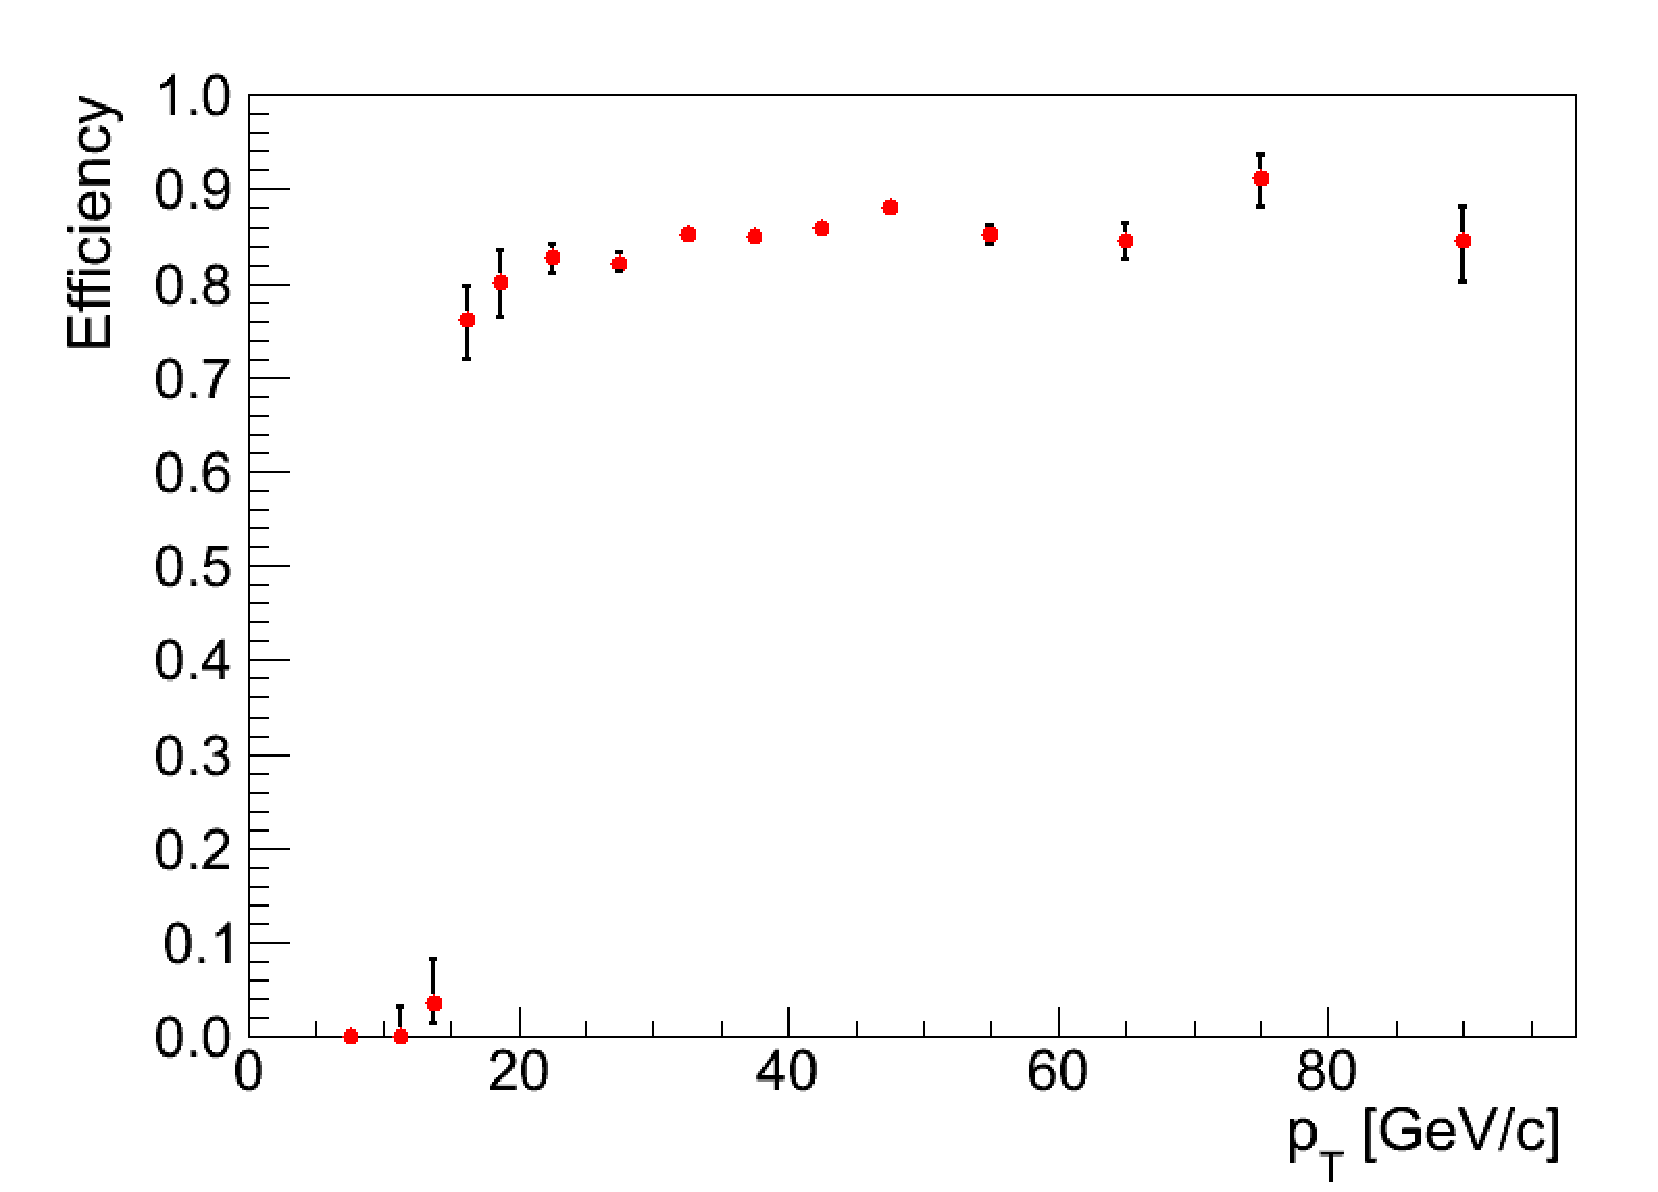
\includegraphics[width=0.48\textwidth]{figures/MuonTriggerEffVsPt_SingleMu15_v1.pdf}}
%\subfigure[PromptReco v1]{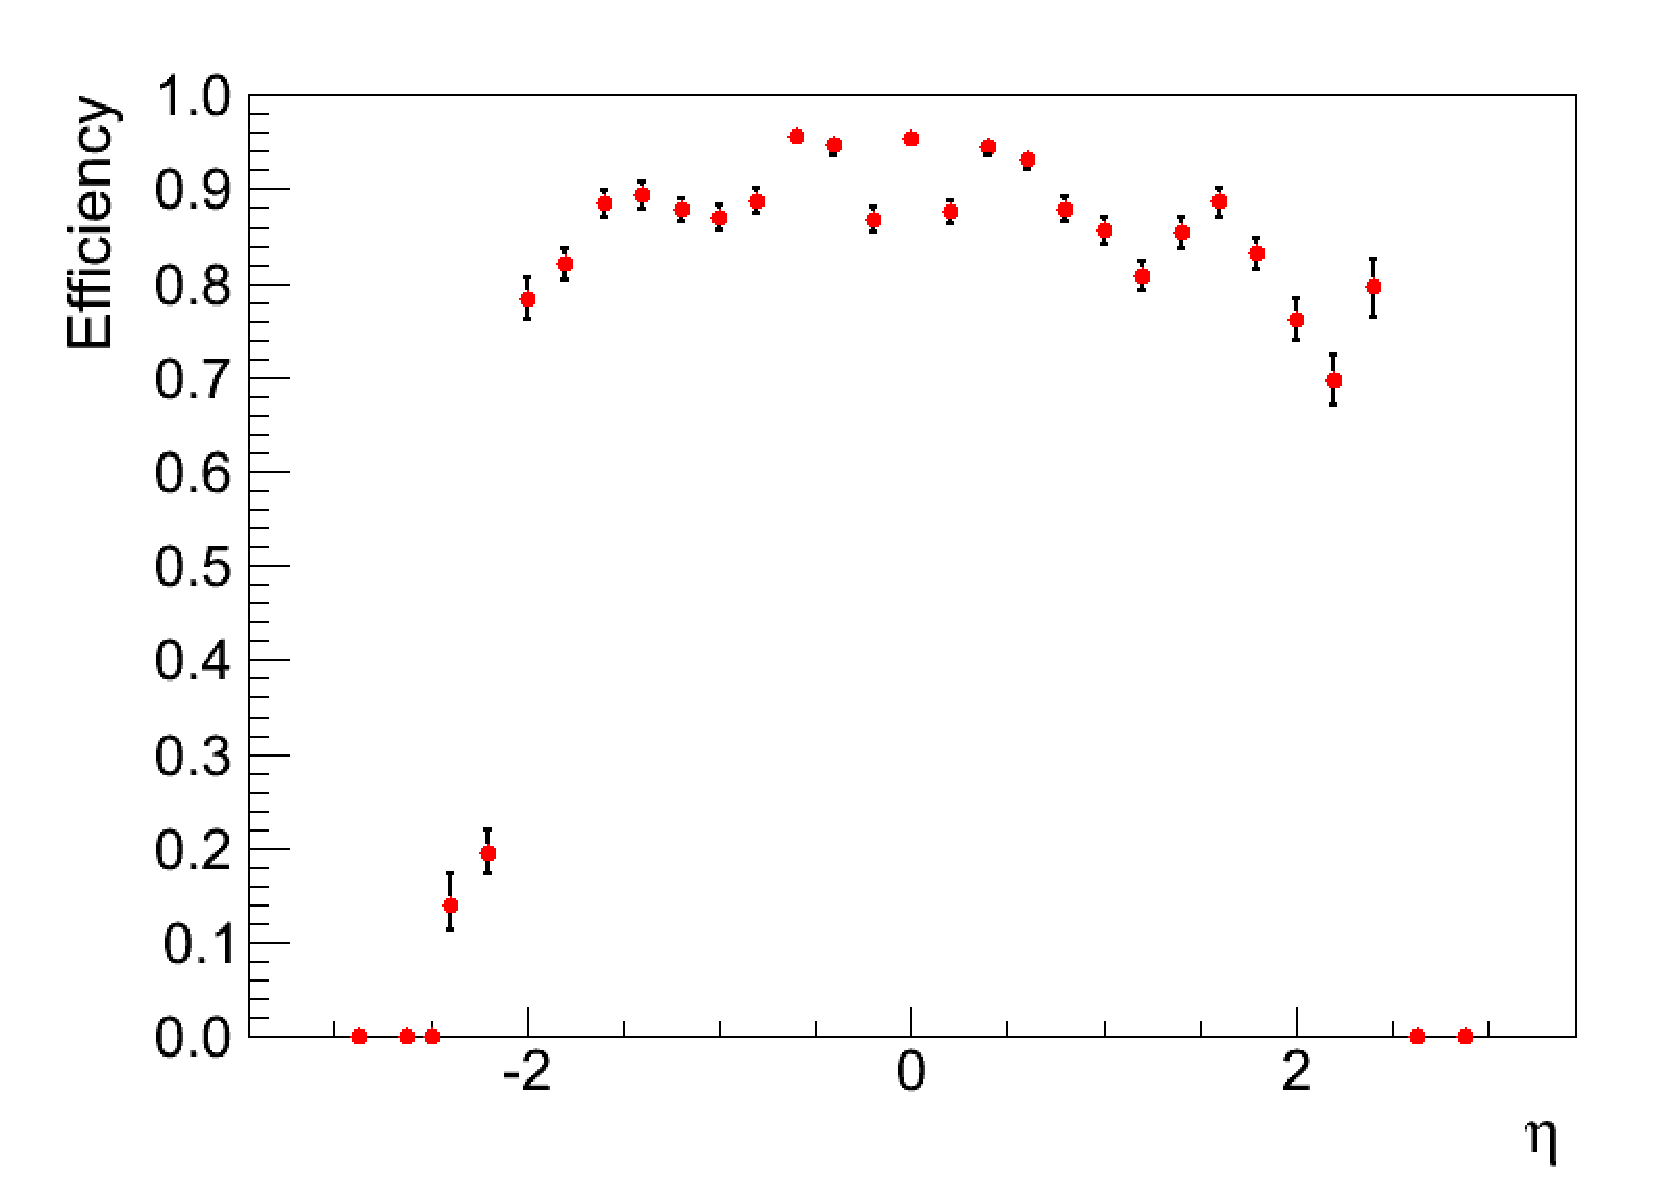
\includegraphics[width=0.48\textwidth]{figures/MuonTriggerEffVsEta_SingleMu15_v1.pdf}}
%\subfigure[PromptReco v2]{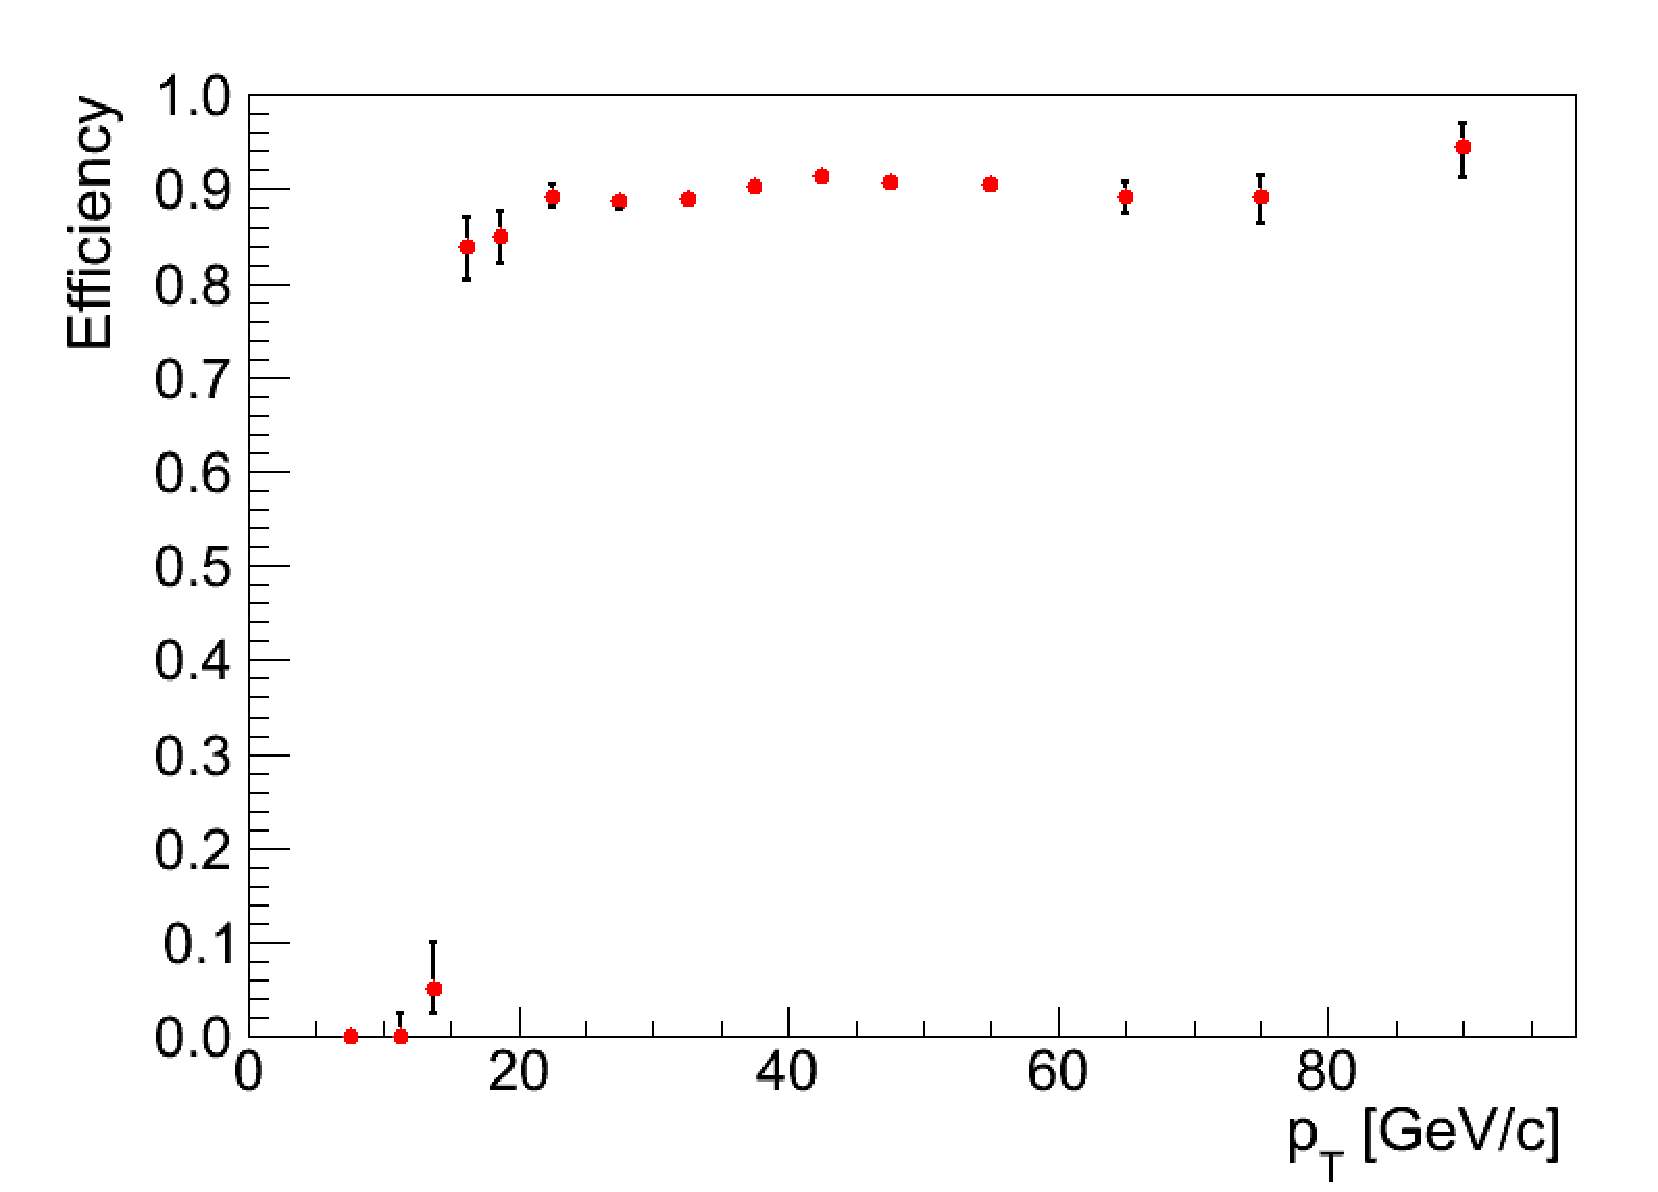
\includegraphics[width=0.48\textwidth]{figures/MuonTriggerEffVsPt_SingleMu15_v2.pdf}}
%\subfigure[PromptReco v2]{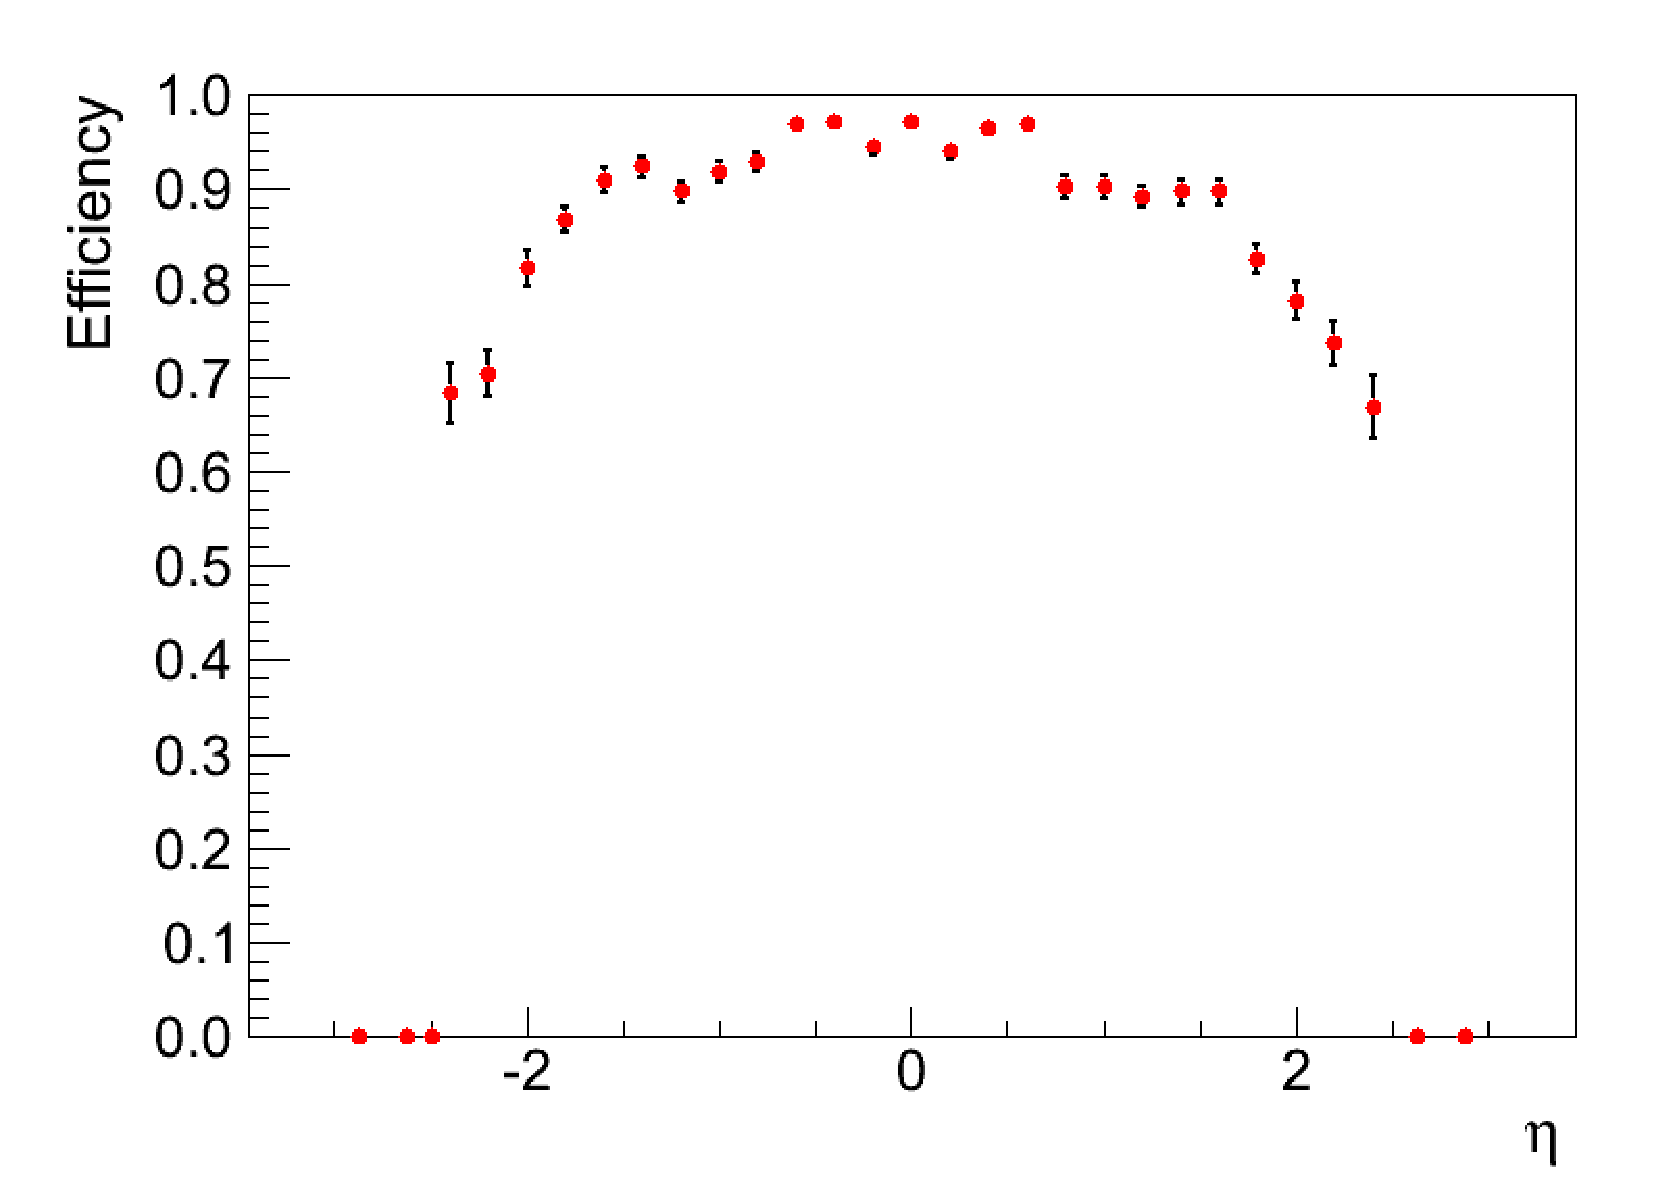
\includegraphics[width=0.48\textwidth]{figures/MuonTriggerEffVsEta_SingleMu15_v2.pdf}}
%\end{center}
%\caption{Efficiency for the single muon trigger as a function of $p_{T}$ and $\eta$ for
%two different primary dataset eras.}
%\label{fig:SingleMu15TriggerEfficiency}
%\end{figure} 
%
%
%
%\begin{figure}[!ht]
%\begin{center}
%\subfigure[PromptReco v1]{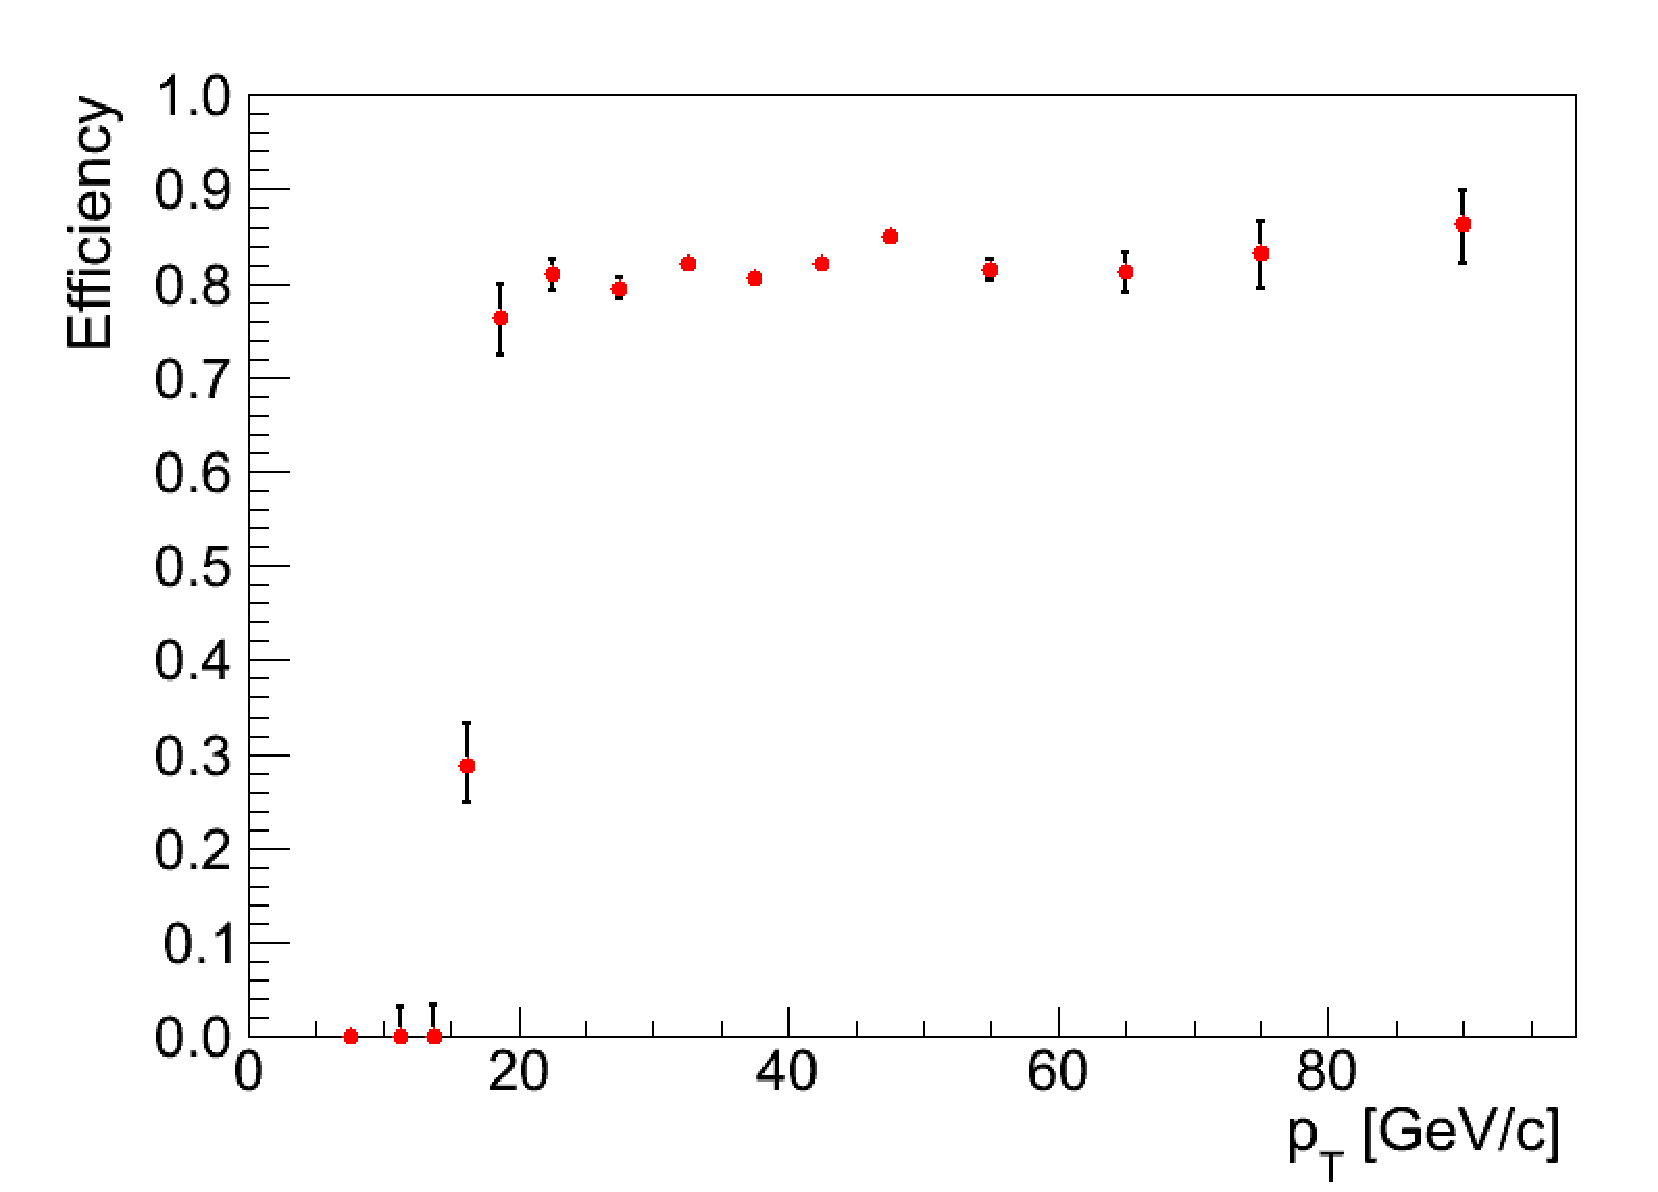
\includegraphics[width=0.48\textwidth]{figures/MuonTriggerEffVsPt_SingleIsoMu17_v1.pdf}}
%\subfigure[PromptReco v1]{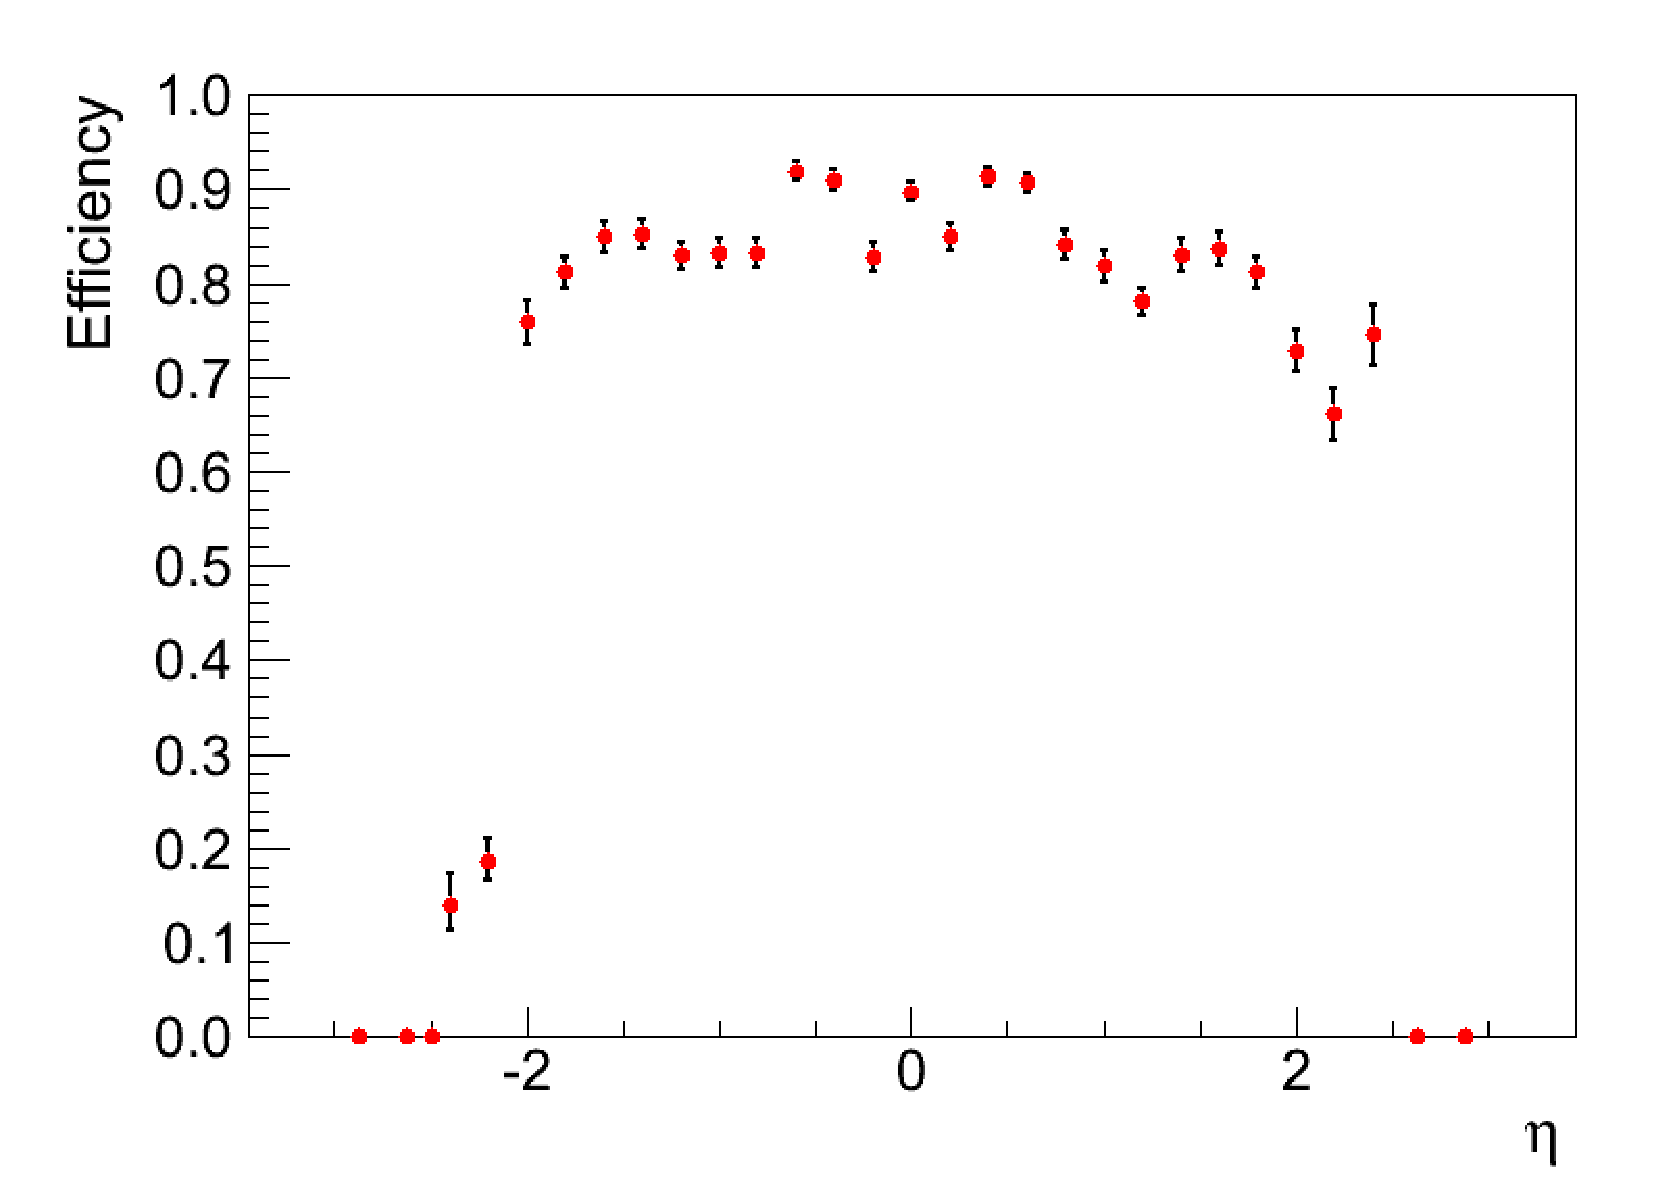
\includegraphics[width=0.48\textwidth]{figures/MuonTriggerEffVsEta_SingleIsoMu17_v1.pdf}}
%\subfigure[PromptReco v2]{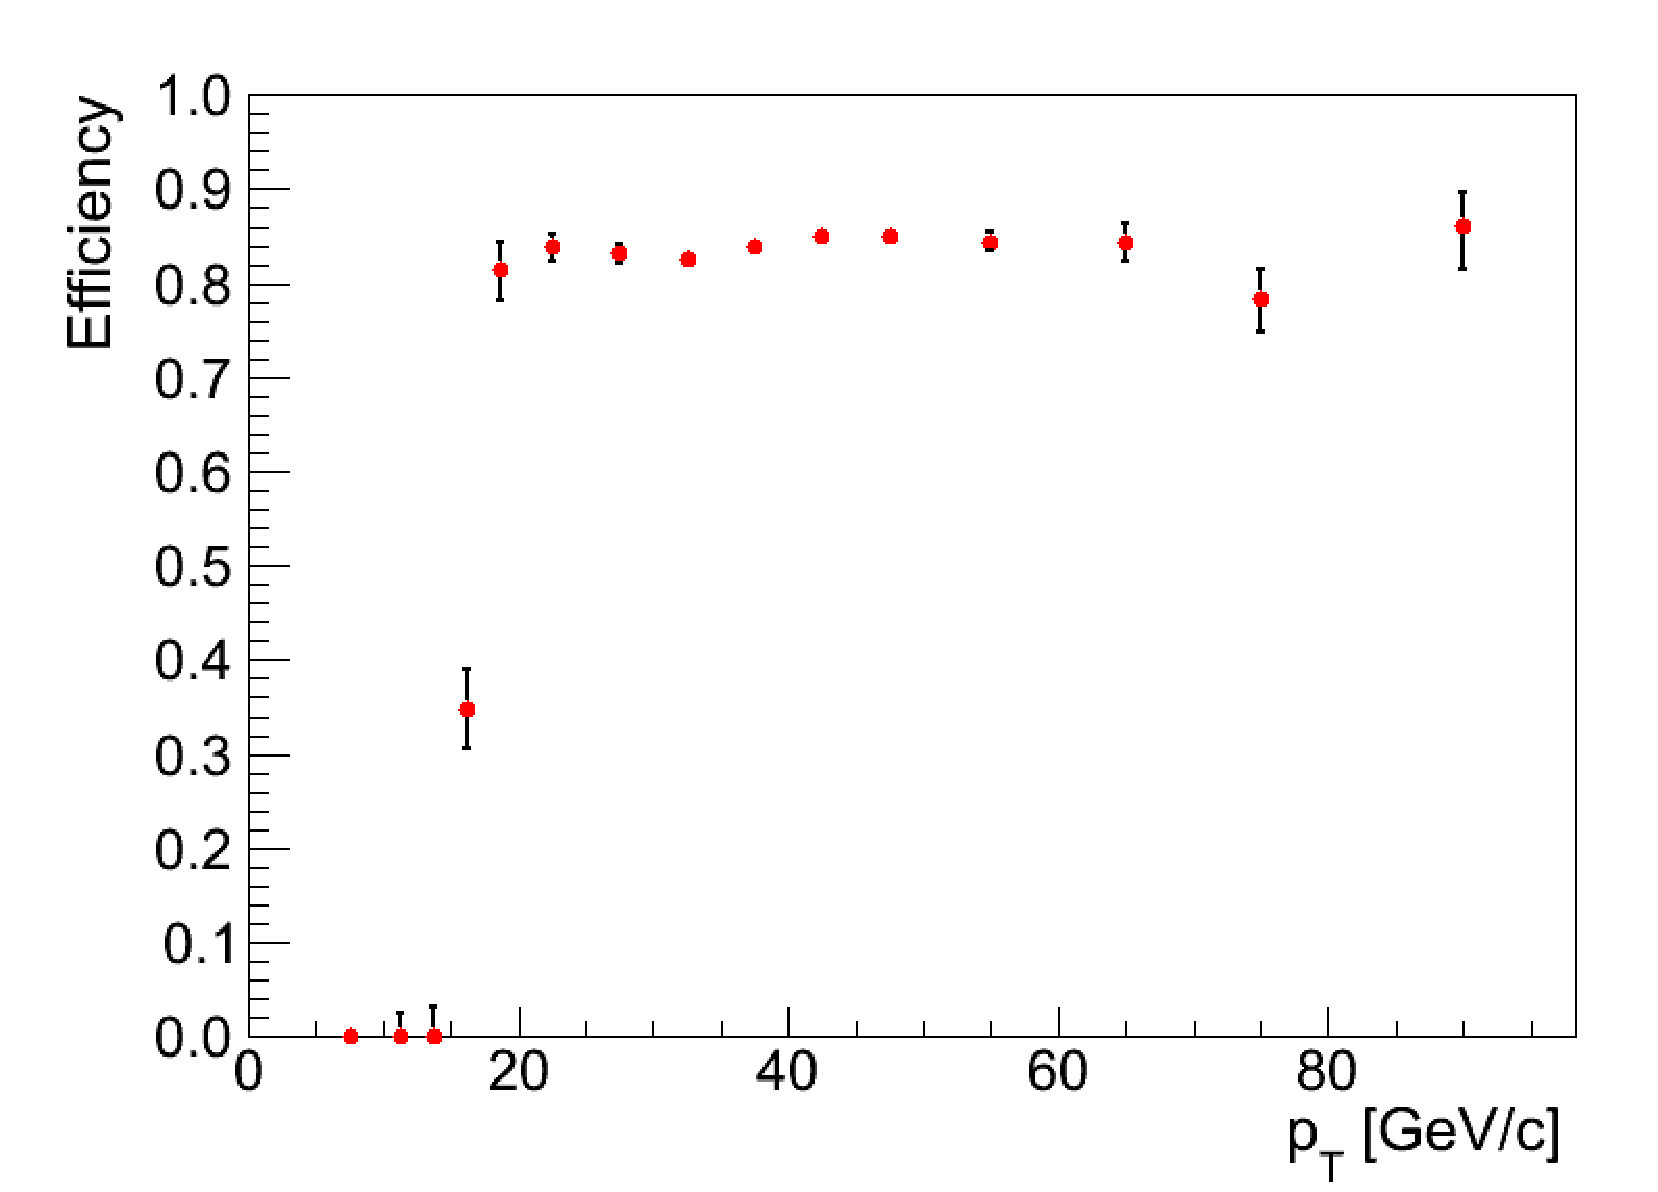
\includegraphics[width=0.48\textwidth]{figures/MuonTriggerEffVsPt_SingleIsoMu17_v2.pdf}}
%\subfigure[PromptReco v2]{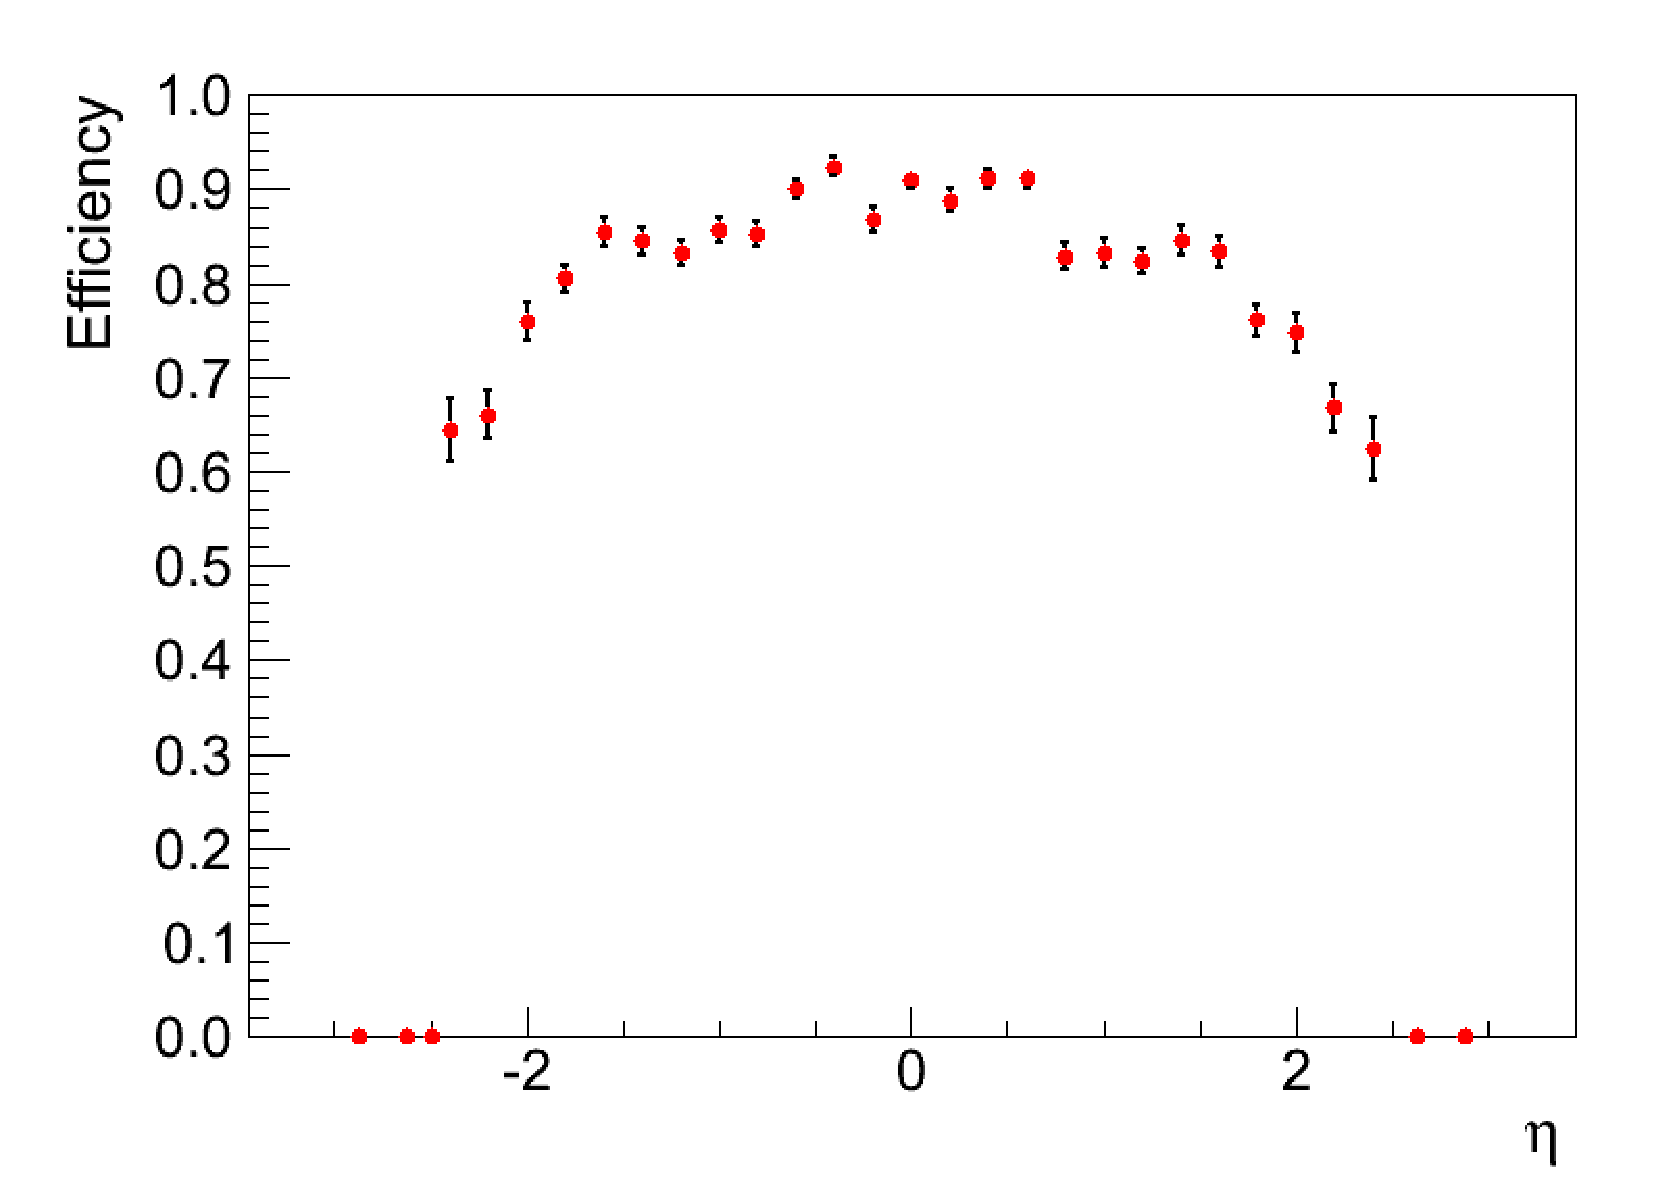
\includegraphics[width=0.48\textwidth]{figures/MuonTriggerEffVsEta_SingleIsoMu17_v2.pdf}}
%\end{center}
%\caption{Efficiency for the single isolated muon trigger as a function of $p_{T}$ and $\eta$ for
%two different primary dataset eras.}
%\label{fig:SingleIsoMu17TriggerEfficiency}
%\end{figure} 
%
%\begin{table}[!ht]
%\begin{center}
%\begin{tabular}{c|c|c} 
%\hline
%\multicolumn{3}{c}{PromptReco v1}                                \\
%\hline
%              & Barrel ( $|\eta|<1.5$ )  & Endcap ( $|\eta|>1.5$ ) \\  
%\hline
%\hline
%10$<p_{T}<$15 & 0.966 + 0.029 - 0.075  & 0.960 + 0.033 - 0.086     \\  \hline
%15$<p_{T}<$20 & 0.967 + 0.018 - 0.031  & 0.950 + 0.027 - 0.046     \\  \hline
%20$<p_{T}$   & 0.955 + 0.003 - 0.003  & 0.947 + 0.005 - 0.005      \\
%\hline
%\hline
%\multicolumn{3}{c}{PromptReco v2}                                \\
%\hline
%              & Barrel ( $|\eta|<1.5$ )  & Endcap ( $|\eta|>1.5$ ) \\  
%\hline
%\hline
%10$<p_{T}<$15 & 1.000 + 0.000 - 0.053  & 1.000 + 0.000 - 0.059     \\  \hline
%15$<p_{T}<$20 & 0.974 + 0.014 - 0.024  & 0.945 + 0.030 - 0.050     \\  \hline
%20$<p_{T}$   & 0.966 + 0.002 - 0.002  & 0.952 + 0.004 - 0.005      \\
%\hline
%\end{tabular}
%\caption{Per muon efficiency for HLT\_DoubleMu7.}
%\label{tab:eff_double_mu}
%\end{center}
%\end{table}
%
%\begin{figure}[!ht]
%\begin{center}
%\subfigure[PromptReco v1]{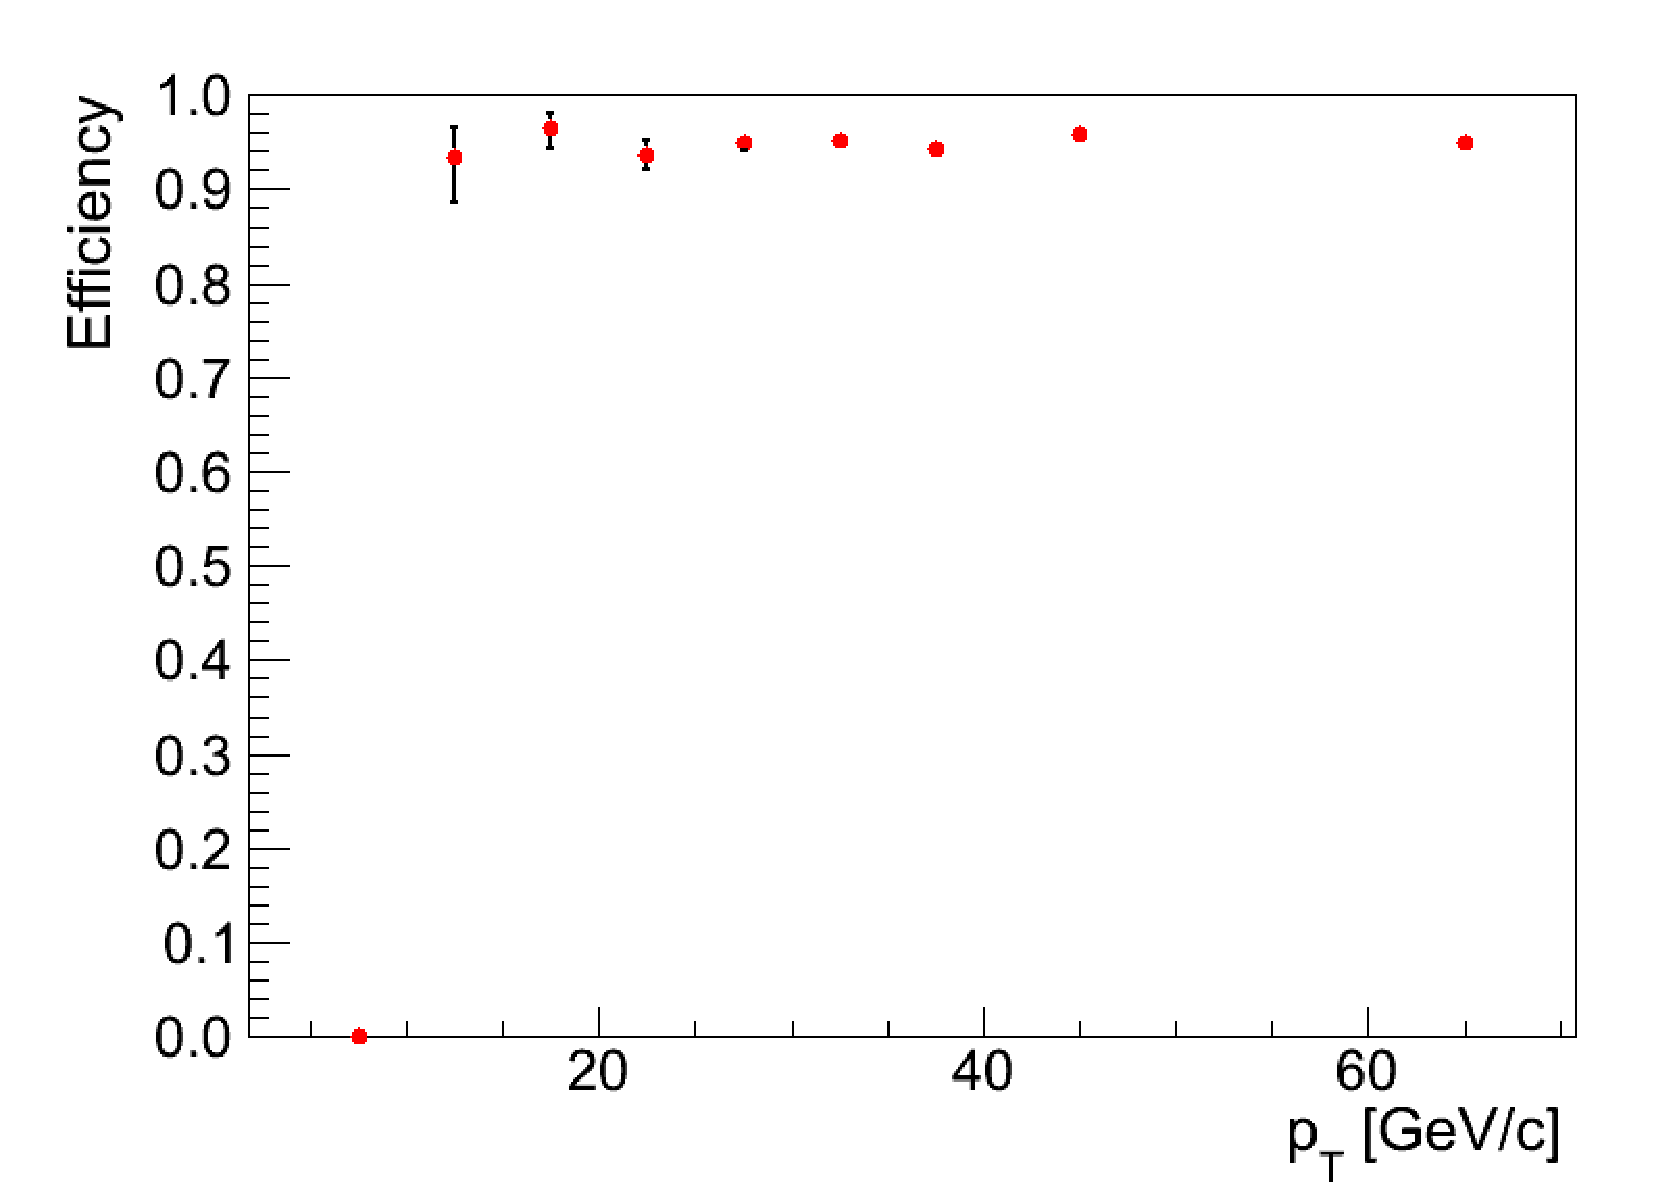
\includegraphics[width=0.48\textwidth]{figures/MuonTriggerEffVsPt_DoubleMu7_v1.pdf}}
%\subfigure[PromptReco v1]{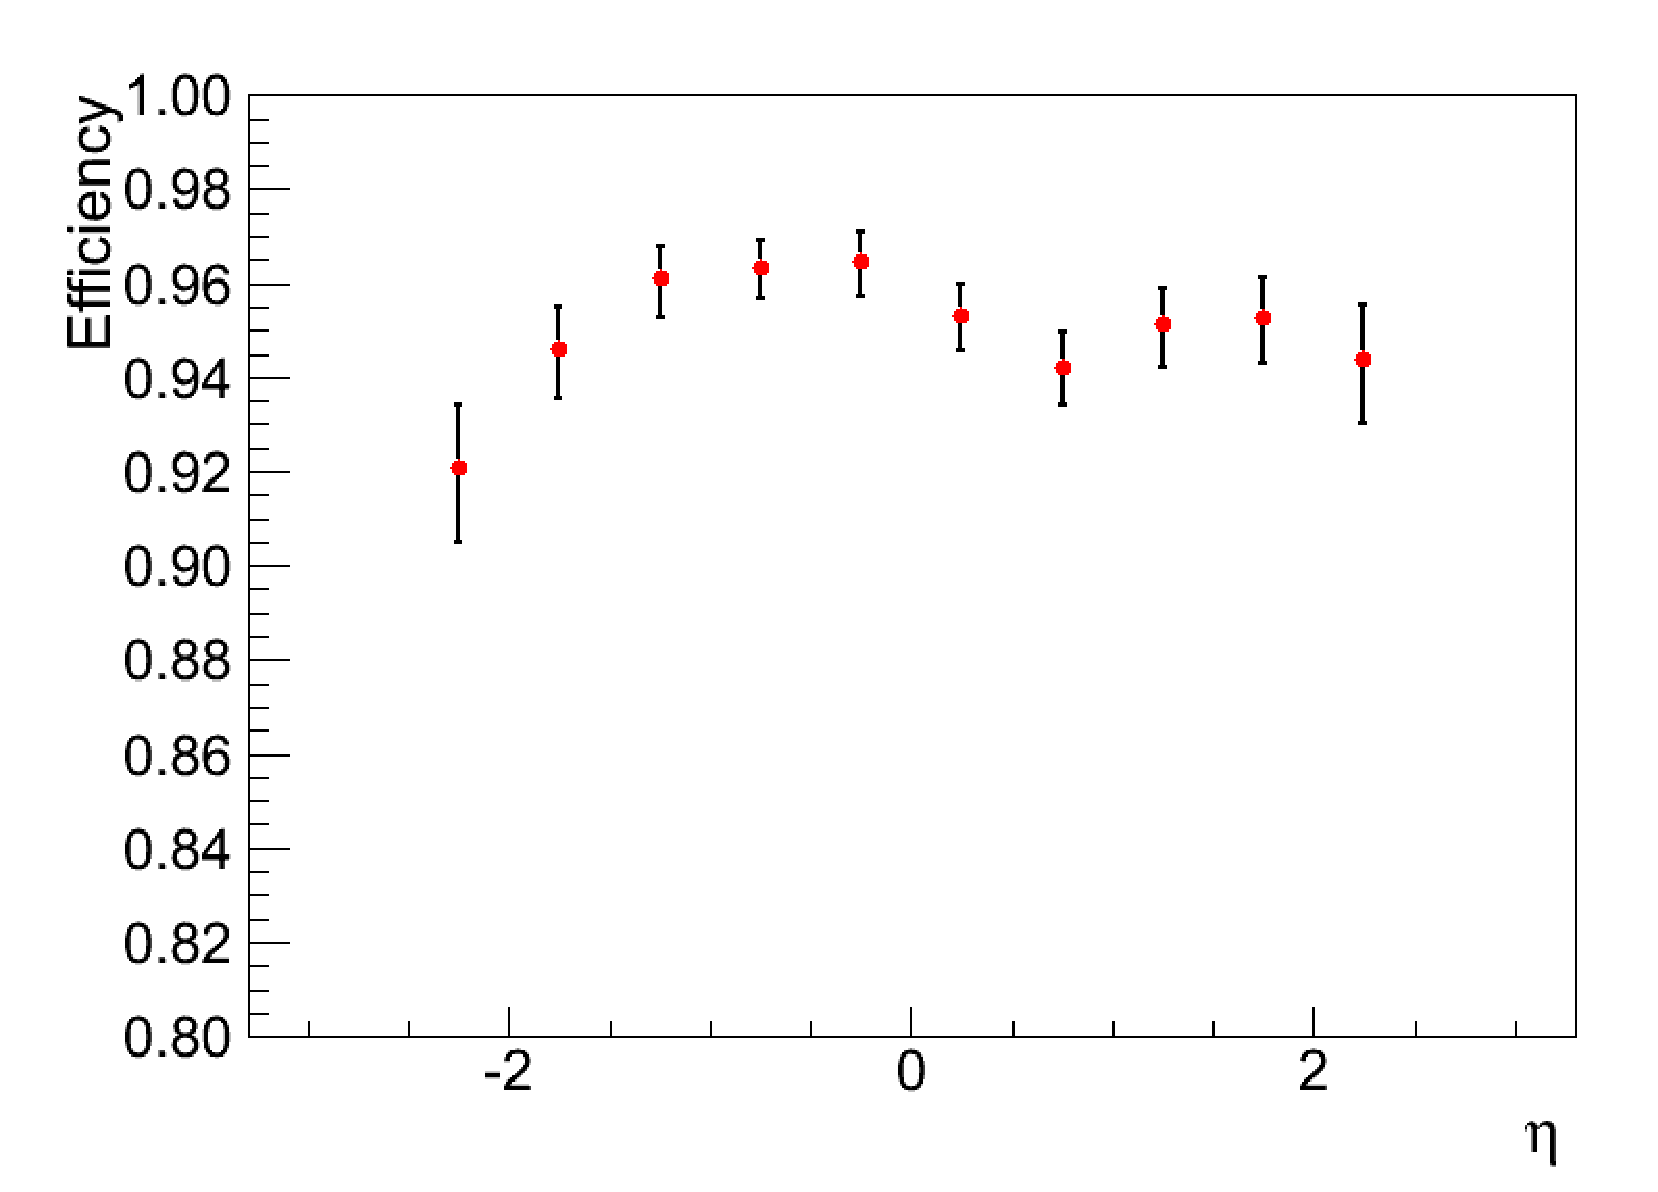
\includegraphics[width=0.48\textwidth]{figures/MuonTriggerEffVsEta_DoubleMu7_v1.pdf}}
%\subfigure[PromptReco v2]{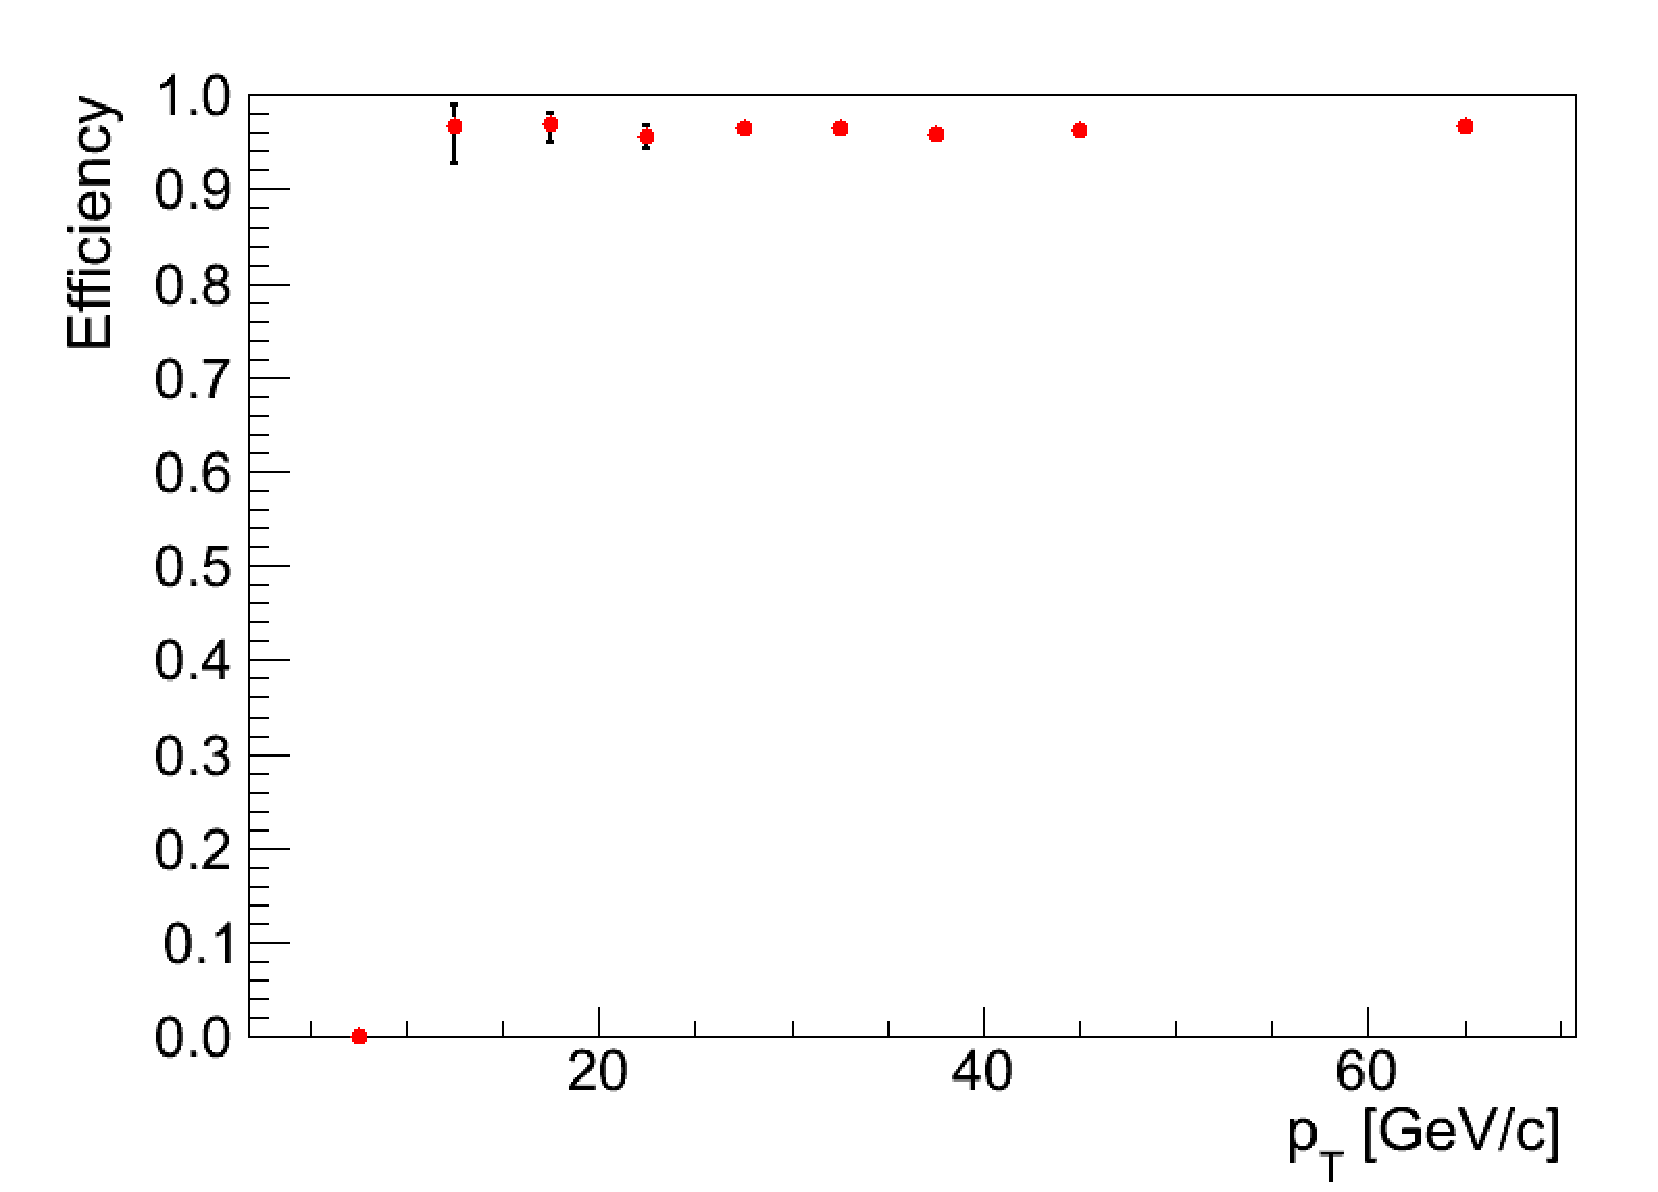
\includegraphics[width=0.48\textwidth]{figures/MuonTriggerEffVsPt_DoubleMu7_v2.pdf}}
%\subfigure[PromptReco v2]{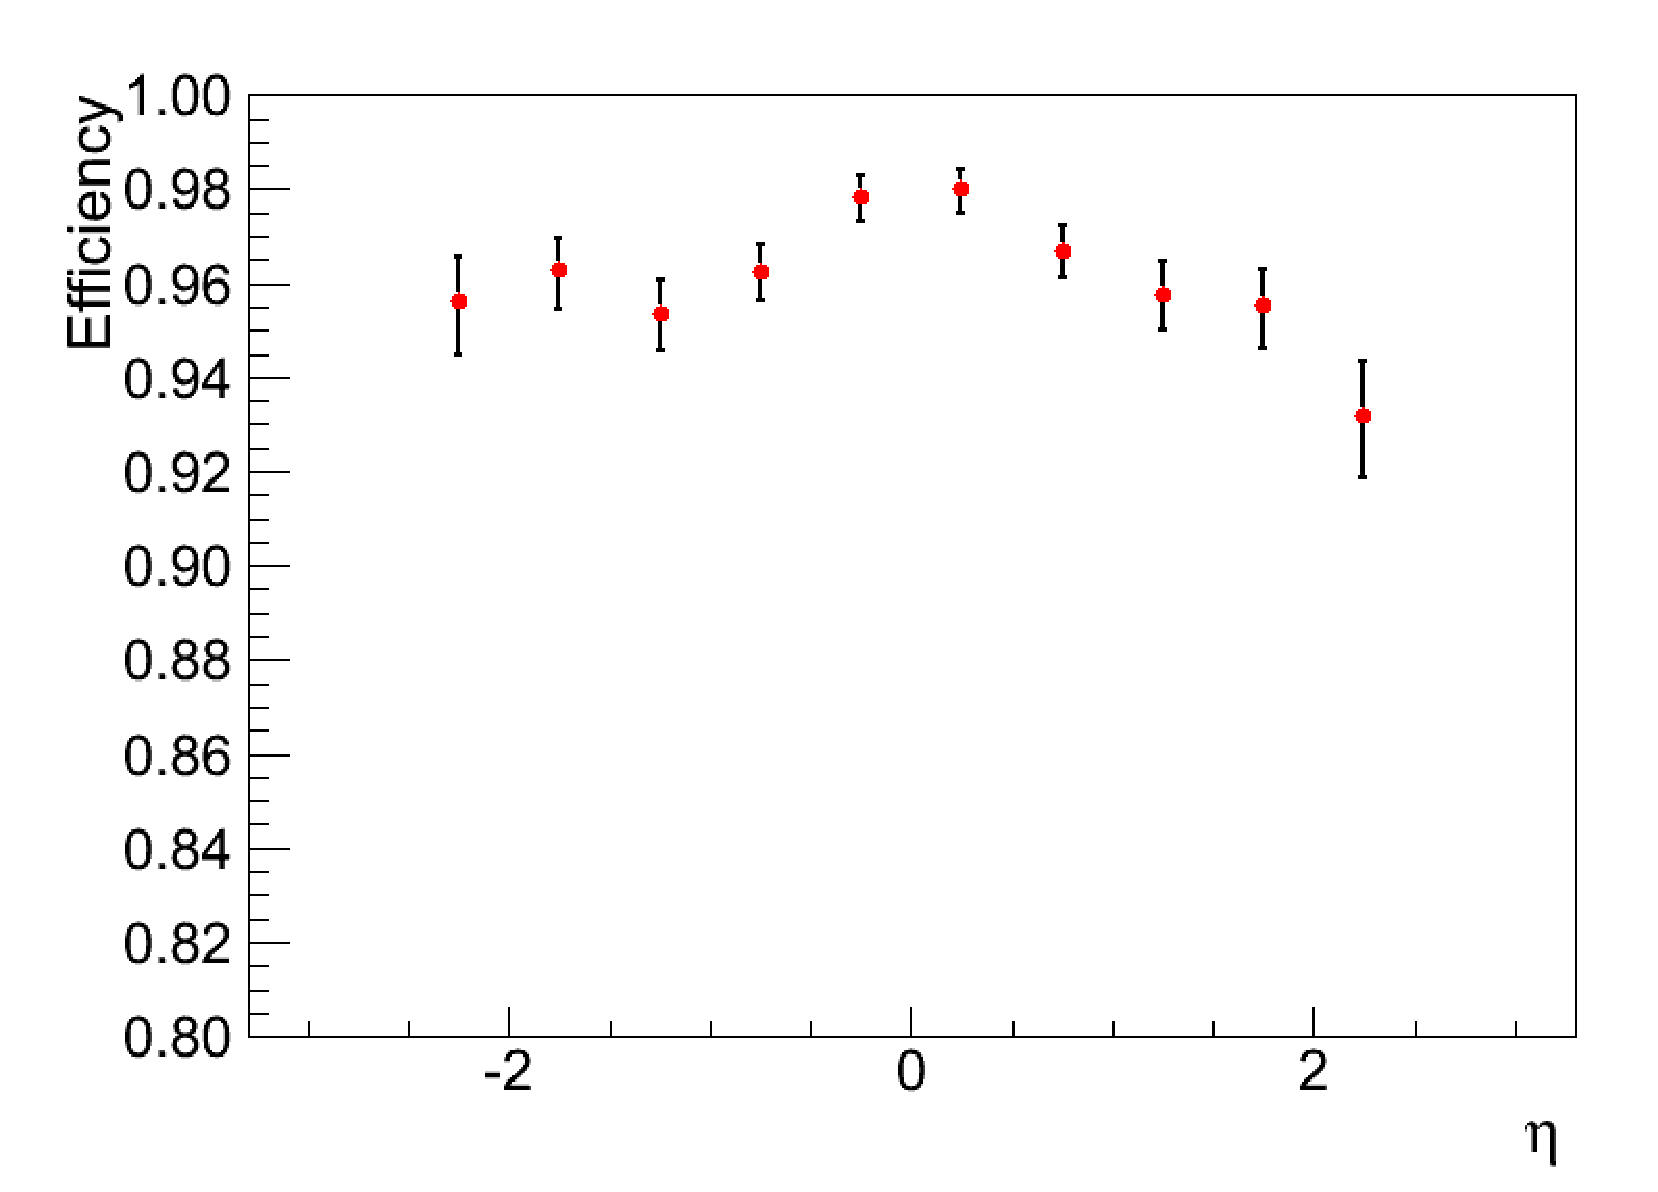
\includegraphics[width=0.48\textwidth]{figures/MuonTriggerEffVsEta_DoubleMu7_v2.pdf}}
%\end{center}
%\caption{Efficiency for one leg of the double muon trigger as a function of $p_{T}$ and $\eta$ for
%two different primary dataset eras.}
%\label{fig:DoubleMu7TriggerEfficiency}
%\end{figure} 
%
%The muon trigger efficiency with respect to muons passing the offline
%selection is summarized in Table \ref{tab:eff_single_mu} and
%\ref{tab:eff_single_isomu} for the single muon {HLT\_Mu15} and
%single isolated muon {HLT\_IsoMu17} triggers respectively.
%We show the single muon trigger efficiencies for two periods of data taking,
%because the first period was affected by a bug in the Level-1 trigger logic,
%which is clearly visible as an inefficiency in the negative endcap region.
%
%\begin{table}[!ht]
%\begin{center}
%\begin{tabular}{c|c|c}
%\hline
%\multicolumn{3}{c}{PromptReco v1}                                \\
%\hline
%              & Barrel ( $|\eta|<1.5$ )  & Endcap ( $|\eta|>1.5$ ) \\
%\hline
%\hline
%10$<p_{T}<$15 & 0.000 + 0.031 - 0.000  & 0.000 + 0.032 - 0.000     \\  \hline
%15$<p_{T}<$20 & 0.587 + 0.039 - 0.040  & 0.462 + 0.050 - 0.049     \\  \hline
%20$<p_{T}$   & 0.860 + 0.003 - 0.003  & 0.709 + 0.007 - 0.007      \\
%\hline
%\hline
%\multicolumn{3}{c}{PromptReco v2}                                \\
%\hline
%              & Barrel ( $|\eta|<1.5$ )  & Endcap ( $|\eta|>1.5$ ) \\
%\hline
%\hline
%10$<p_{T}<$15 & 0.000 + 0.027 - 0.000  & 0.000 + 0.027 - 0.000     \\  \hline
%15$<p_{T}<$20 & 0.648 + 0.034 - 0.035  & 0.529 + 0.049 - 0.050     \\  \hline
%20$<p_{T}$   & 0.873 + 0.003 - 0.003  & 0.758 + 0.006 - 0.006      \\
%\hline
%\end{tabular}
%\caption{Per muon efficiency for HLT\_IsoMu17.}
%\label{tab:eff_single_isomu}
%\end{center}
%\end{table}
%
%\begin{table}[!ht]
%\begin{center}
%\begin{tabular}{c|c|c}
%\hline
%\multicolumn{3}{c}{PromptReco v1}                                \\
%\hline
%              & Barrel ( $|\eta|<1.5$ )  & Endcap ( $|\eta|>1.5$ ) \\
%\hline
%\hline
%10$<p_{T}<$15 & 0.017 + 0.038 - 0.014  & 0.018 + 0.040 - 0.015     \\  \hline
%15$<p_{T}<$20 & 0.860 + 0.026 - 0.031  & 0.664 + 0.046 - 0.049     \\  \hline
%20$<p_{T}$    & 0.898 + 0.003 - 0.003  & 0.736 + 0.007 - 0.007     \\
%\hline
%\hline
%\multicolumn{3}{c}{PromptReco v2}                                \\
%\hline
%              & Barrel ( $|\eta|<1.5$ )  & Endcap ( $|\eta|>1.5$ ) \\
%\hline
%\hline
%10$<p_{T}<$15 & 0.015 + 0.033 - 0.012  & 0.030 + 0.039 - 0.020     \\  \hline
%15$<p_{T}<$20 & 0.918 + 0.019 - 0.023  & 0.714 + 0.043 - 0.047     \\  \hline
%20$<p_{T}$    & 0.937 + 0.002 - 0.002  & 0.813 + 0.006 - 0.006     \\
%\hline
%\end{tabular}
%\caption{Per muon efficiency for HLT\_Mu15.}
%\label{tab:eff_single_mu}
%\end{center}
%\end{table}

Having measured the per lepton trigger efficiency,
it is necessary to compute the expected efficiency for dilepton events to pass the trigger.
This is done by taking into account the $p_{T}$ and $\eta$ distributions
of both leptons in the signal sample. The expected efficiencies are used to scale
the Monte Carlo on an event-by-event basis. Since the triggers involve different $p_T$ 
thresholds and lepton flavour combinations, for each final state ($ee$, $e\mu$, and $\mu\mu$)
the overall dilepton efficiency is derived from a weighted average of the 
efficiencies from the various trigger paths. For a pair of selected leptons of flavour $\ell$ and $\ell'$
with kinematics $(p_T,\:\eta)$ and $(p'_T,\:\eta')$, 

\begin{equation}
\varepsilon_{\ell\ell'}(p_T,\:\eta,\:p'_T,\:\eta') = \sum_i f_i\cdot\varepsilon_i(p_T,\:\eta,\:\ell,\:p'_T,\:\eta',\:\ell'),
\end{equation}

where the summation index $i$ runs over all the trigger paths used to obtain the signal sample and $f_i$
is the weight of the contribution to the overall efficiency from each trigger.

The determination of $f_i$ comes from the fraction of selected events in data which came 
through that trigger path. For example, if $10\%$ of the selected $\mu\mu$ events were triggered 
by HLT\_IsoMu17, then the overall efficiency for $\mu\mu$ events will include the efficiency 
of HLT\_IsoMu17 weighted by $f_i=0.1$. There is no ambiguity in the assignment of a selected event to
a trigger since the trigger requirements are applied in a mutually exclusive way: the selection is
performed by checking each trigger sequentially and requiring that an event passing a trigger
must not have also passed another trigger previously in the sequence.

For each trigger path, the determination of $\varepsilon_i$ from the measured single leg efficiencies depends
on whether the trigger is a single or a double lepton trigger. For a single lepton trigger,

\begin{equation}
\varepsilon_{single}(p_T,\:\eta,\:\ell',\:p'_T,\:\eta',\:\ell') = 
1 - \left(1-\varepsilon_{leg}(p_T,\:\eta)\right)\left(1-\varepsilon_{leg}(p'_T,\:\eta')\right),
\end{equation}

whereas for a double lepton trigger,

\begin{equation}
\varepsilon_{double}(p_T,\:\eta,\:\ell',\:p'_T,\:\eta',\:\ell') = \varepsilon_{leg}(p_T,\:\eta)\cdot\varepsilon_{leg}(p'_T,\:\eta').
\end{equation}

If there is a mismatch of lepton flavour with the trigger (e.g. $\ell=e$ and $i=$HLT\_IsoMu17) then $\varepsilon_{leg}=0$.
